\pagestyle{mystyle}

\part{物理约束与智能方法融合}

\renewcommand{\parttitle}{物理约束与智能方法融合}

\chapter{智能启发式搜索与算法优化}

引力波数据分析的核心挑战之一，是在一个极其庞大的算法设计空间中寻找高性能的信号处理策略。匹配滤波依赖预先构建的波形模板库，其最优性以已知信号形态和高斯平稳噪声假设为前提；深度神经网络虽然弱化了显式模板依赖，却通常增加了可解释性和校准验证的难度。本章探讨第三条路线：将大语言模型（LLM）的领域知识生成能力与结构化进化搜索相结合，实现对引力波检测算法的自动发现。这一路线的核心优势在于，所发现的算法由可检视的代码组成，其决策逻辑更容易接受物理学家的审查和验证。

\section{算法设计作为搜索问题}

引力波信号处理管道通常由若干功能模块串联构成：数据白化、时频变换、跨探测器相干统计量构造、阈值判决等。每个模块的具体实现——选用何种滤波器、如何组合多探测器信息、采用何种统计量——都对应一个离散的设计选择。将所有可能的模块组合视为一个搜索空间，引力波检测算法的设计问题便转化为：在该空间中找到使某一性能指标（如敏感距离 AUC）最大化的程序~\cite{schafer2023mlgwsc1}。

这一视角揭示了传统方法在大规模组合搜索中的局限。手工设计依赖专家经验，容易受既有知识结构和探索能力约束；网格搜索在组合爆炸面前迅速失效；遗传编程虽能自动搜索，却若缺乏领域知识引导，往往生成大量物理上无意义的候选。大语言模型的出现为这一问题提供了新的可能~\cite{romera2024funsearch}：LLM 在预训练阶段接触过大量科学和工程文本，能够生成语法正确且部分物理上合理的候选算法，从而将搜索空间从“任意可能的程序”压缩到“更可能有物理意义的程序”这一较小子集。

\subsection{AutoML 与神经架构搜索的启示}

在算法设计自动化领域，自动机器学习（AutoML）和神经架构搜索（NAS）是两条已有成熟实践的技术路线。AutoML 通过自动化超参数搜索——包括贝叶斯优化、进化算法和强化学习等策略——大幅减少了模型调优所需的人工干预。在图像分类基准任务上，NAS 自动发现的网络架构（如 DARTS 和 EfficientNet 系列）曾在 ImageNet 等基准上取得有竞争力的结果，说明算法设计空间的系统性搜索能够发现人类专家难以直接想到的高效结构。

然而，将这些成功经验直接移植到科学计算领域时，面临一系列本质性的新挑战。首先，评估函数的计算代价远高于图像分类。引力波检测性能的标准指标——误报率下的敏感距离曲线（FAR-sensitive distance curve）——需要在大量真实或模拟噪声数据上统计计算，单次评估耗时30至60秒（在 GPU 加速条件下），是图像分类准确率评估的数百倍。其次，设计空间包含领域特定的物理约束，这些约束对通用搜索算法并不透明：白化操作必须正确估计并消除噪声的功率谱密度，跨探测器相干统计量的构造必须尊重引力波在两个探测器间的时间延迟关系（最大10毫秒），匹配滤波的实现必须处理非平稳噪声的短时变化。通用 NAS 方法在这样的约束空间中搜索，极易生成物理上无意义的候选，浪费宝贵的评估配额。

\subsection{引力波管道的模块化形式化描述}

为了将算法设计问题纳入严格的数学框架，我们首先建立引力波信号处理管道的模块化形式化描述。一个典型的引力波检测管道可以抽象为一系列函数的复合：
\begin{equation}
f_{\text{detect}} = f_n \circ f_{n-1} \circ \cdots \circ f_2 \circ f_1,
\end{equation}
其中每个 $f_i$ 对应一个具体的处理步骤。以 MLGWSC-1 标准管道为例，$f_1$ 可能是白化操作，$f_2$ 是时频变换（可以是 Q 变换、短时傅里叶变换 STFT 或连续小波变换 CWT），$f_3$ 是跨探测器相干统计量的构造，$f_4$ 是对统计量的平滑与阈值判决。每个步骤不仅有若干可选的实现方式，还有多个可调的连续参数——白化的基线长度、时频变换的窗口宽度和重叠率、相干统计量的时延搜索范围等。

这一形式化描述揭示了搜索空间的组合爆炸性质。若每个步骤有 $k$ 种可选实现，各有 $m$ 个离散可调参数，则整个管道的搜索空间大小约为 $O(k^n \cdot m^{n \cdot p})$，其中 $p$ 是每步参数数量。即便取保守估计（$n=5$，$k=4$，$m=3$，$p=3$），搜索空间大小已超过 $10^{10}$，远超任何穷举策略的可行范围。更重要的是，这一搜索空间中绝大多数点对应物理上无意义的管道——例如，跳过白化步骤直接对原始数据应用匹配滤波会使非平稳噪声干扰信号检测；逆序执行步骤（先阈值判决后时频变换）在信号处理上没有意义。因此，高效搜索的关键在于如何利用领域知识约束搜索空间，而非盲目枚举。

\subsection{程序搜索的数学框架}

将管道搜索问题形式化为黑箱优化，可以写成：
\begin{equation}
\theta^* = \arg\max_{\theta \in \Theta} \mathcal{F}(\text{code}(\theta)),
\end{equation}
其中 $\theta$ 是描述管道结构（模块选择和组合方式）的参数向量，$\text{code}(\theta)$ 是由 $\theta$ 描述的可执行程序，$\mathcal{F}$ 是评估函数（在 MLGWSC-1 上即为敏感距离 AUC），$\Theta$ 是所有物理上合理的参数配置的集合。

这一框架与标准超参数优化的本质区别在于：$\theta$ 是离散的程序结构参数，而非连续的实数向量。这使得基于梯度的优化方法（如 Adam、SGD）无法直接应用——因为 $\text{code}(\theta)$ 关于 $\theta$ 的梯度在离散空间中无法定义。即便将结构参数松弛到连续空间（类似 DARTS 的做法），引力波评估函数 $\mathcal{F}$ 的高计算代价也使得梯度估计（需要对每个参数进行有限差分近似）在实践中不可行。

这一分析确立了为何需要无梯度的黑箱优化策略——进化算法和贝叶斯优化是两类自然的候选。但如下文所展示的，在科学计算领域，这两类通用策略还需要与领域知识深度结合，才能在有限的评估预算内找到高性能的解。

从更宏观的视角来看，将算法设计问题视为搜索问题这一框架转换，本身就具有重要的认识论意义。传统的算法设计隐含着一种以人类专家为中心的知识创造模式：算法的每一步改进都是研究者通过分析现有方法的局限、结合物理直觉、设计新的解决方案，再通过实验验证的结果。这一过程的效率上限由人类研究者的认知带宽决定，且存在系统性的认知偏见——研究者倾向于探索自己熟悉的算法结构空间（如CNN架构或匹配滤波变体），而难以主动探索与已有知识结构差异较大的“陌生”算法组合。将算法设计形式化为黑箱优化问题，则将人类专家从“主动设计者”转变为“问题定义者”和“评估者”——专家负责定义性能指标（MLGWSC-1敏感距离）、注入领域约束（物理约束提示词）、以及审查搜索结果的物理合理性，而算法空间的探索则由LLM驱动的自动搜索完成。这一角色转变不是对专家知识的替代，而是对专家时间和注意力的重新分配：从在算法细节上反复试错，到在高层次的问题定义和物理约束上投入更多精力。在引力波信号处理这一涉及深厚物理知识的领域，这种人机协作模式将人类专家的物理洞察、约束识别与结果验证能力，同人工智能系统的高并发搜索和系统性探索能力结合起来，代表了引力波人工智能研究方法论的重要演进方向。

\section{LLM驱动的自动启发式设计}

将 LLM 与进化搜索结合用于自动算法发现，近年来形成了一条清晰的方法演进脉络。

\textbf{FunSearch}~\cite{romera2024funsearch} 是这一范式的奠基性工作。Google DeepMind 于 2023 年在 \textit{Nature} 上报告，FunSearch 将预训练 LLM 与自动评估器配对，在程序空间中进行进化搜索。LLM 负责生成多样化的候选程序，评估器过滤错误输出并防止幻觉传播，进化机制在高分程序之间进行重组。FunSearch 在极值组合数学的 cap set 问题上发现了改进既有构造的新方案，说明 LLM 驱动的程序搜索有可能在严格评估器约束下产生具有科学价值的候选结果。

\textbf{EoH}（Evolution of Heuristics）~\cite{liu2024eoh} 将这一思路推进到启发式算法设计领域。EoH 的关键创新在于引入双层进化：不仅进化可执行代码，还同时进化描述启发式设计思路的自然语言（“thought”）。LLM 将思路翻译为代码，进化操作同时作用于两个层次。在在线装箱、旅行商等组合优化基准上，EoH 超越了人工设计的启发式算法。

\textbf{ReEvo}（Reflective Evolution）~\cite{ye2024reevo} 进一步引入“反思”机制。ReEvo 让 LLM 分析高分与低分候选之间的差异，生成“语言梯度”（verbal gradient）——一种以自然语言表达的改进方向——从而为进化搜索提供更有针对性的引导。ReEvo 在 TSP（旅行商问题）、CVRP（有容量约束的车辆路径问题）等多个 NP-hard 问题上取得了较强的 LLM-based AHD 基准结果。

上述方法均针对组合优化问题，其候选解为离散决策序列，评估函数定义明确。引力波信号处理问题则呈现出本质不同的挑战：候选解是连续参数优化的信号处理管道，需要满足物理约束，且评估指标（敏感距离 AUC）的计算涉及真实噪声数据，代价较高。这些差异促使了 Evo-MCTS 框架的提出。

从 FunSearch 到 EoH 到 ReEvo 再到 Evo-MCTS 的演进轨迹，体现了 LLM 驱动自动算法发现方法论的快速发展。这一演进可以从三个维度来理解：第一，知识注入的深化——FunSearch 使用通用领域知识，EoH 引入问题特定的设计思路，ReEvo 加入比较性学习（分析高分vs低分的差异），Evo-MCTS 引入深度领域专业知识（物理约束、信号处理原则）；第二，搜索结构的完善——从简单进化库（FunSearch）到思路-代码双层结构（EoH），再到MCTS树结构的多尺度探索（Evo-MCTS），搜索空间的导航越来越有组织；第三，应用场景的复杂化——从纯数学问题（cap set）到离散优化（TSP、CVRP）再到物理科学计算（引力波检测），候选解的约束越来越多，评估函数越来越复杂。这一演进表明，LLM 驱动的自动算法发现正在从相对清晰的基准问题向更复杂的实际问题推进。Evo-MCTS 在引力波这一高度专业化的科学计算问题上的表现，是这一推进过程中的一个案例，也提示类似框架未来有必要在更广泛的科学计算领域接受系统检验。

\subsection{FunSearch 的工作流程细节}

FunSearch 的核心架构由三个相互协作的组件构成。评估器（evaluator）对每个候选程序运行沙箱测试，返回性能分数，并过滤语法错误和运行时错误——这一过滤机制至关重要，因为 LLM 生成的代码有相当比例存在语法错误或逻辑缺陷，若不过滤则会污染进化库。进化库（program database）维护当前高分程序的集合，按性能和多样性双重标准排序：仅保留高分程序会导致多样性丧失，而仅保留多样程序则会浪费评估配额在低质量候选上。LLM 在看到库中的高分程序和相关问题描述后，生成改进版本；这一“看到优良候选后改进”的机制类似于人类专家在阅读前人工作后提出改进方案的认知过程。

在 cap set 问题上，FunSearch 找到了 $n=8$ 时大小为 $512$ 的 cap set（此前已知构造为 $509$），是由 LLM 驱动的程序搜索发现数学新构造的代表性案例。这一结果的意义不仅在于数值上的改进，更在于说明 LLM 驱动的搜索有可能在严格评估器约束下发现人类专家尚未系统探索的结构——这为将类似方法应用于科学计算中的算法发现提供了有力先例。

\subsection{EoH 的双层进化机制}

EoH 的核心创新在于将启发式算法的“设计意图”与“具体实现”解耦，并在两个层次上同时进行进化。自然语言描述（“thought”）编码了启发式算法的设计意图，例如“优先选择约束最强的变量”或“在局部搜索中优先探索高密度区域”。LLM 将这些自然语言描述翻译为可执行的 Python 代码，形成候选启发式算法。

进化算子同时作用于 thought 和 code 两个层面。思路层面的交叉操作将两个算法的设计意图合并（例如“结合 A 的约束优先策略和 B 的密度感知策略”），由 LLM 翻译成新的代码实现；代码层面的变异操作直接修改代码的局部结构，保留整体设计意图。这种双层进化使得搜索能够在高层语义空间（设计思路）和低层实现空间（代码细节）之间协同探索，避免了单纯代码进化中常见的“语义漂移”问题——即代码在形式上发生变化但实际功能退化。

在在线装箱（online bin packing）问题上，EoH 生成的启发式在标准测试集上比人工设计的 best-fit-decreasing 算法好约 3\%。这一提升看似不大，但考虑到 best-fit-decreasing 是经过长期优化的经典算法，EoH 在有限搜索预算内取得可比并略优的结果具有重要的方法论意义。

\subsection{ReEvo 的语言梯度机制}

ReEvo 的核心创新是“语言梯度”（verbal gradient）概念。在标准梯度下降中，梯度向量指示了参数空间中性能提升最快的方向；在离散的程序空间中，梯度无法直接定义，但 ReEvo 通过 LLM 的语言理解能力构造了一种类似的引导信号。

具体地，对高分候选 $p^+$ 和低分候选 $p^-$，ReEvo 提示 LLM 分析“为什么 $p^+$ 比 $p^-$ 更好？”。LLM 生成的文本描述指出两者的关键差异——例如“$p^+$ 在局部搜索阶段使用了更细粒度的邻域结构，而 $p^-$ 的邻域过于粗糙导致错过了局部最优”——这一描述作为下一轮改进的方向，引导 LLM 生成融合 $p^+$ 优点并修正 $p^-$ 缺陷的新候选。

这种机制类似于梯度下降，但作用在离散的程序空间上，且“梯度”以人类可读的自然语言形式表达，具有内在的可解释性。在 TSP 上，ReEvo 生成的构造启发式比 LKH3 竞争性算法只差约 1\%（此前 LLM 方法与 LKH3 的差距约为 10\%--20\%），显示了语言梯度机制在缩小 LLM 方法与专业求解器差距方面的有效性。

\subsection{从组合优化到科学计算的挑战}

上述三种方法在组合优化领域取得了令人印象深刻的结果，但将其直接应用于引力波检测算法发现时，面临若干本质性的新挑战。

第一，评估函数的统计性质。组合优化问题的评估通常是确定性的：给定输入，解的质量可以精确计算（如 TSP 的路径总长度）。引力波检测的评估涉及统计量——误报率（FAR）和敏感距离是在大量数据上的统计量，单次评估含有不可忽略的随机噪声。这意味着同一算法在不同评估运行中可能得到不同的分数，进化选择机制需要能够处理这种评估噪声，避免将随机高分误认为真正的性能提升。

第二，候选解的混合离散-连续性质。组合优化的解通常是纯离散的决策序列（如 TSP 的城市访问顺序），而引力波管道包含大量连续参数（白化滤波器的截止频率、时频变换的窗口宽度、相干统计量的阈值等）。这些连续参数需要在离散的程序结构搜索之外进行额外的数值优化，形成双层优化问题。

第三，物理约束的隐式性。引力波管道的物理约束（如白化的必要性、相干统计量的时延范围）对通用 LLM 并不透明，需要通过精心设计的提示词将这些约束显式传达给 LLM。这些差异使得通用框架不能直接应用，需要专门适配，这正是 Evo-MCTS 框架设计的出发点。

\section{Evo-MCTS与可解释算法发现}

\textbf{Evo-MCTS}（Evolutionary Monte Carlo Tree Search）~\cite{wang2025evomcts} 是专为科学计算中的算法发现设计的框架，以引力波检测为核心案例研究。其核心思想是将 LLM 的领域知识生成能力、蒙特卡洛树搜索（MCTS）的结构化探索策略，以及进化计算的种群多样性维护机制三者有机整合。

\begin{figure}[htbp]
\centering
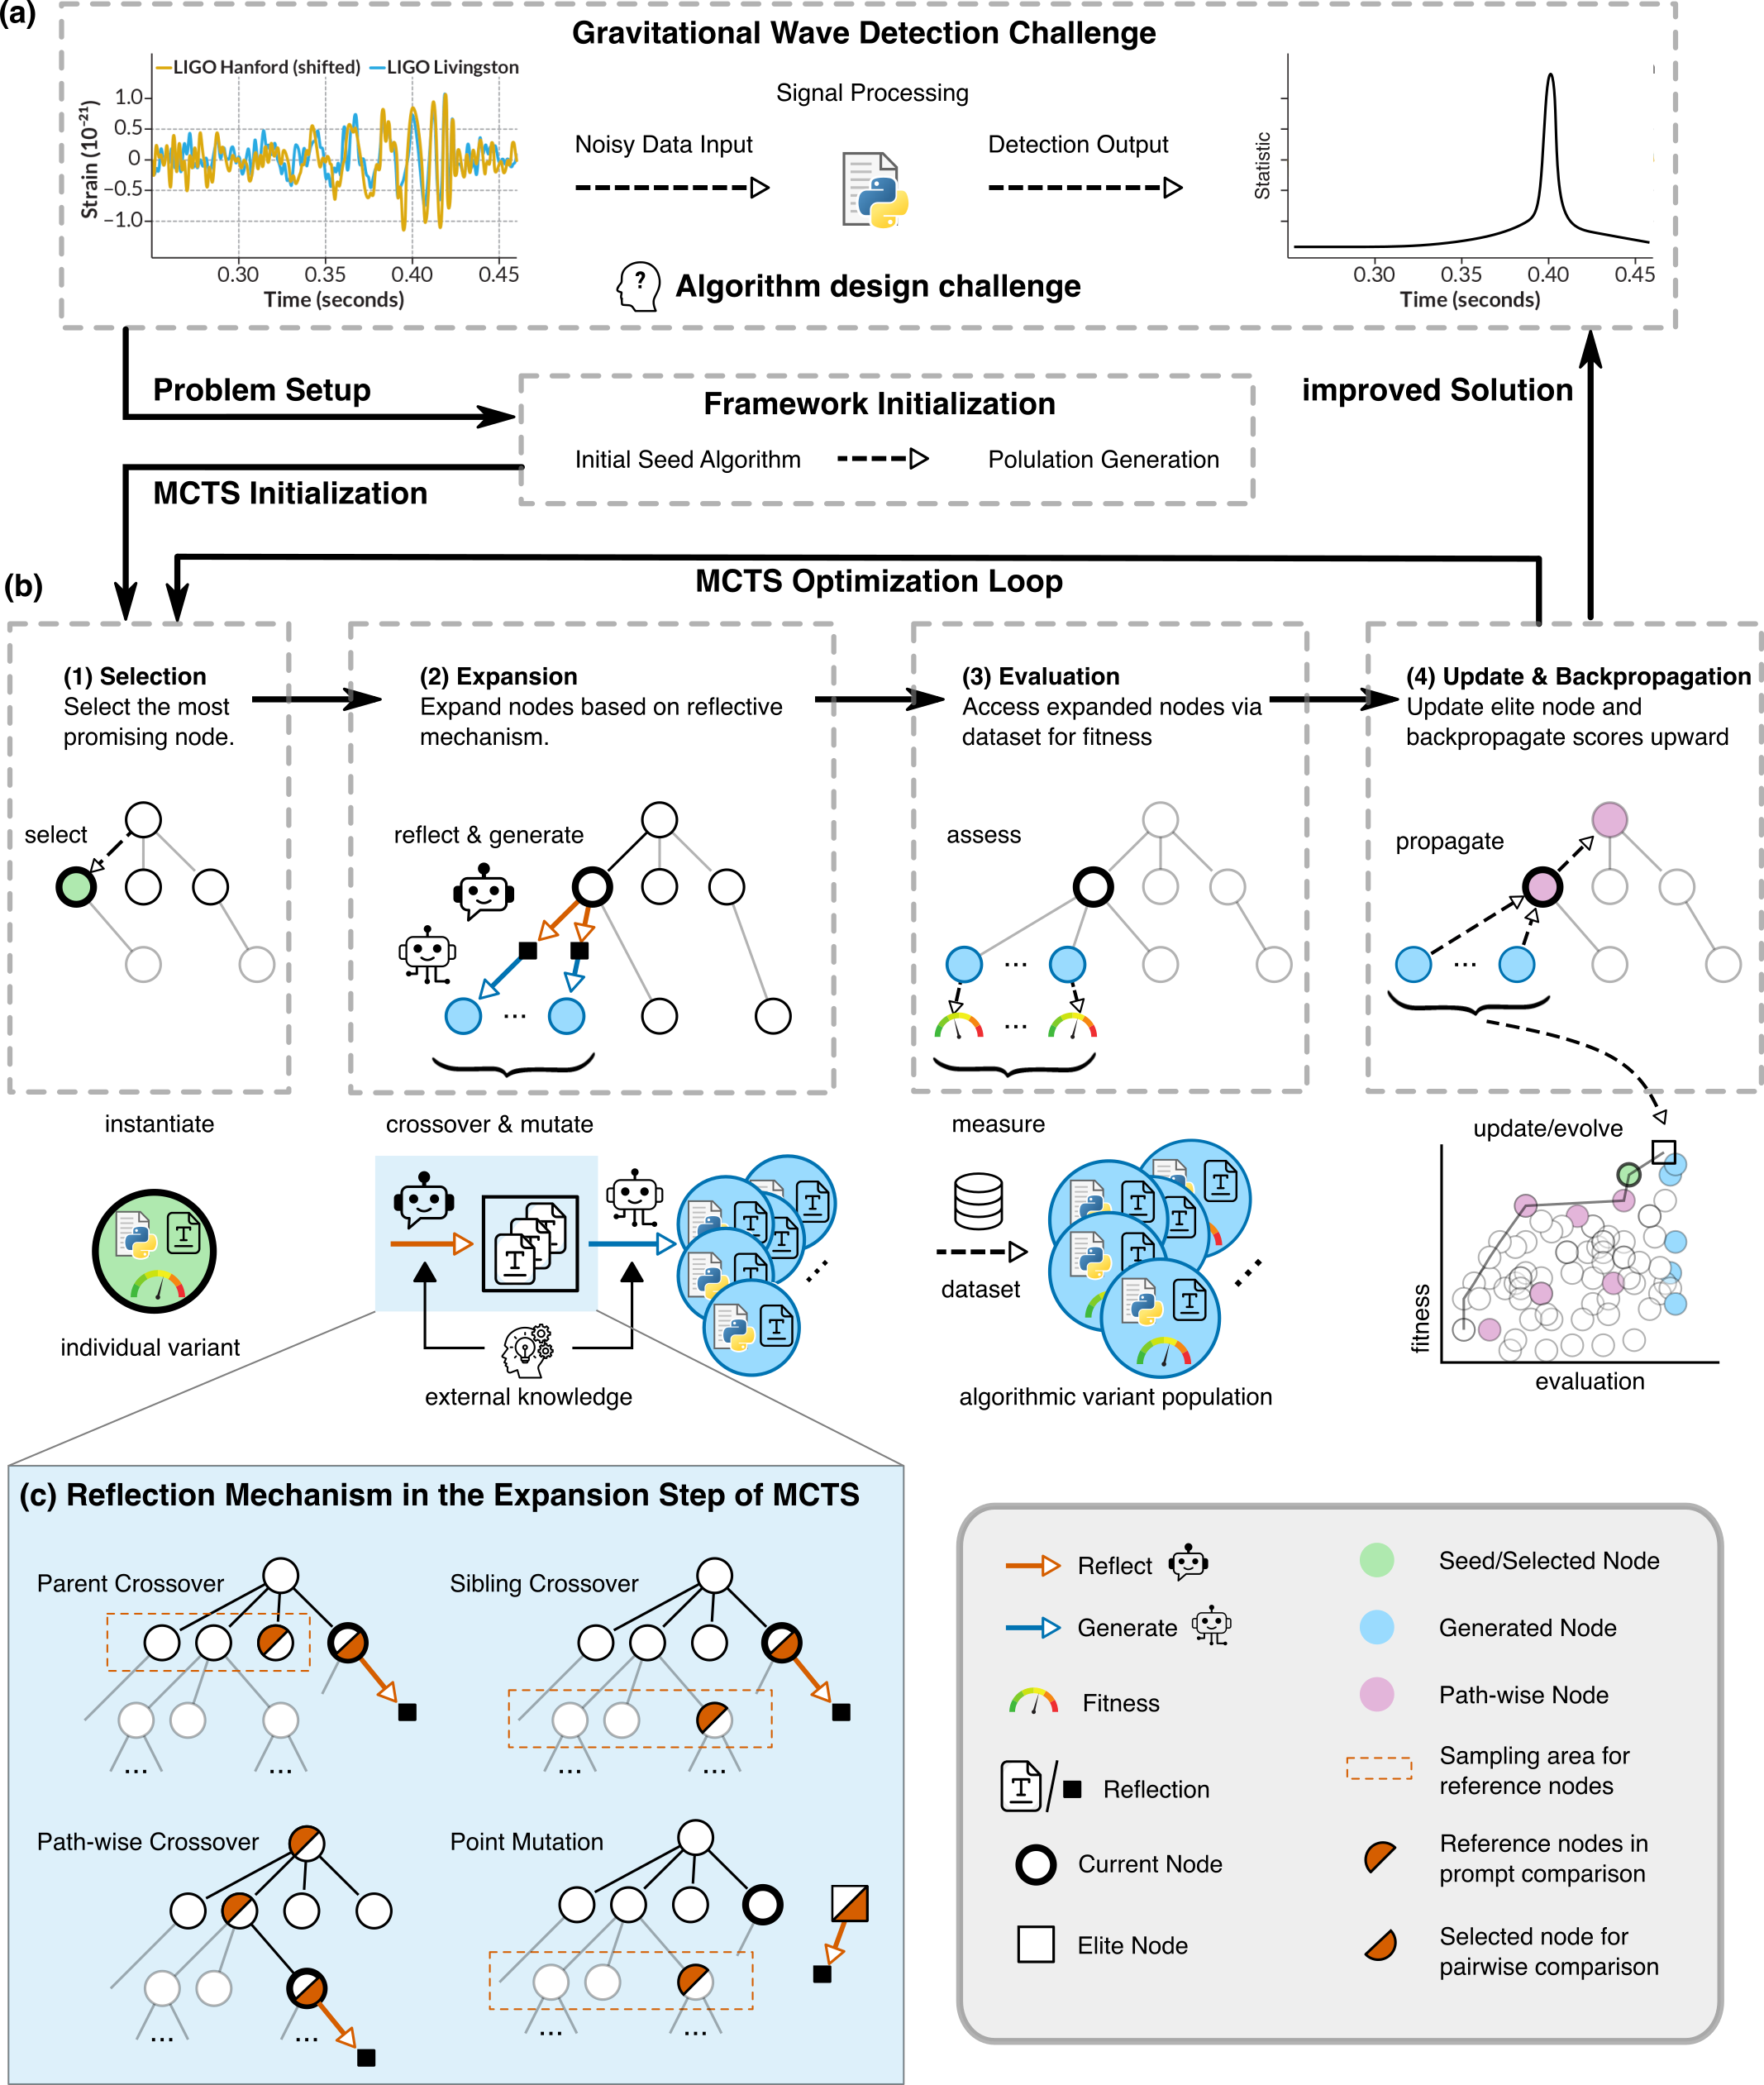
\includegraphics[height=0.72\textheight,keepaspectratio]{figures/EvoMCTS_fig1_framework.png}
\caption{Evo-MCTS 框架总体流程。框架以候选引力波检测程序为搜索对象，利用 LLM 生成和反思候选代码，以 MCTS 树组织探索历史，并通过父节点交叉、兄弟节点交叉、路径级交叉和点突变等操作产生新算法；每个候选解通过 MLGWSC-1 真实噪声基准上的适应度评估获得反馈。图引自 Wang 和 Zeng~\cite{wang2025evomcts} 的 Figure 1。}
\label{fig:evomcts_framework}
\end{figure}

\subsection{框架设计}

Evo-MCTS 包含三项相互增强的核心创新：

\textbf{反射式代码合成}（Reflective Code Synthesis）。LLM 在生成候选算法时，不仅利用通用编程知识，还通过精心设计的提示词（prompt）注入引力波信号处理的领域知识——包括白化的物理意义、跨探测器相干统计量的构造原理、时频分析方法的适用场景等。每次生成后，LLM 还对自身输出进行反思，识别潜在的物理不一致性并迭代修正。消融实验表明，领域知识集成将平均适应度从 1244.50 Mpc 提升至 2670.37 Mpc，提升幅度达 115\%。

\textbf{多尺度进化操作}（Multi-Scale Evolutionary Operations）。Evo-MCTS 在 MCTS 树结构上定义了四种进化操作，作用于结构化代码表示：
\begin{itemize}
  \item \textit{父节点交叉}（Parent Crossover）：重组当前节点与其父节点的算法组件；
  \item \textit{兄弟节点交叉}（Sibling Crossover）：在同层节点间交换功能模块；
  \item \textit{路径级交叉}（Path-wise Crossover）：沿树路径提取并重组多代算法的优秀片段；
  \item \textit{点突变}（Point Mutation）：对单一功能模块进行局部修改。
\end{itemize}
这些操作通过 MCTS 树遍历实现语义感知的算法变换，使搜索能够在保持物理合理性的同时探索多样化的算法结构。

\textbf{可解释算法路径}（Interpretable Algorithm Pathways）。MCTS 树结构自然记录了算法发现的完整演化轨迹。每个节点对应一个具体的算法实现，节点间的父子关系反映了算法改进的逻辑链条。这使得研究者能够事后追溯：哪些技术创新在哪个阶段被引入，各创新对性能的贡献如何量化。这一特性在深度神经网络方法中是缺失的。

\subsection{提示词设计与领域知识注入}

Evo-MCTS 的提示词设计是框架成功的关键工程要素之一。每次 LLM 调用的提示词模板包含五个主要部分，共约 2000--3000 个 token。

第一部分是任务描述，明确说明目标任务（MLGWSC-1 Dataset 4 上的引力波检测）、评估规则（敏感距离 AUC 的计算方式）和代码接口规范（输入输出格式、允许使用的库）。这一部分确保 LLM 生成的代码能够被评估器正确执行，避免接口不匹配导致的无效评估。

第二部分是物理约束说明，包括：引力波信号的基本特征（啁啾结构、时频演化、双探测器时延）；探测器噪声的统计特性（非平稳、非高斯、存在线谱噪声）；白化操作的必要性和正确实现方式；跨探测器相干统计量的物理意义和构造原则。这一部分将引力波物理学的核心知识以 LLM 可理解的自然语言形式传达，是领域知识集成的核心载体。

第三部分是当前高分算法代码，作为 LLM 改进的起点。提供具体的代码而非抽象描述，使 LLM 能够在已有成果的基础上进行有针对性的改进，而非从零开始生成。这一设计体现了“站在巨人肩膀上”的搜索策略。

第四部分是性能反馈，包括当前算法在测试集上的敏感距离数值、与基线的对比、以及通过分析识别出的性能瓶颈（例如“在低信噪比区间的检测率偏低”或“对进动信号的适应性不足”）。这一反馈使 LLM 能够有针对性地改进算法的薄弱环节。

第五部分是改进方向建议，基于领域知识提供具体的改进思路（例如“考虑使用更短的白化基线以适应噪声的短时非平稳性”或“尝试引入连续小波变换以捕获信号的时频局部特征”）。这些建议不是强制约束，而是引导 LLM 在物理上有意义的方向上探索。

\subsection{UCB 在 MCTS 中的适配}

蒙特卡洛树搜索（MCTS）的核心是上置信界（UCB）策略，用于平衡探索（exploration）和利用（exploitation）之间的权衡。标准 MCTS 使用 UCT（Upper Confidence Bound for Trees）公式：
\begin{equation}
\text{UCT}(v) = Q(v) + c \sqrt{\frac{\ln N(p(v))}{N(v)}},
\end{equation}
其中 $Q(v)$ 是节点 $v$ 的平均奖励（对应该节点算法的平均敏感距离），$N(v)$ 是节点 $v$ 被访问的次数，$N(p(v))$ 是其父节点的访问次数，$c$ 是控制探索-利用权衡的超参数。

在 Evo-MCTS 中，节点奖励是该节点对应算法在 MLGWSC-1 测试集上的敏感距离。UCT 公式的第一项鼓励选择历史表现好的节点（利用），第二项鼓励选择访问次数少的节点（探索）。参数 $c$ 的选择对搜索效率有重要影响：$c$ 过大会导致过度探索，浪费评估配额在低质量节点上；$c$ 过小会导致过早收敛到局部最优。实践中 $c = 1/\sqrt{2}$ 是一个常用的理论推荐值，但在引力波检测任务中，由于评估函数含有统计噪声，适当增大 $c$（增强探索）有助于避免因评估噪声导致的错误收敛。

通过 MCTS 的树结构，算法发现的完整历史被记录为一棵有向树，支持事后分析：哪些节点是搜索的“主干”（被频繁访问），哪些节点是“探索分支”（访问次数少但性能高），哪些节点是“死胡同”（访问后性能未提升）。这种结构化的搜索历史是 Evo-MCTS 可解释性的重要来源。

\begin{figure}[htbp]
\centering
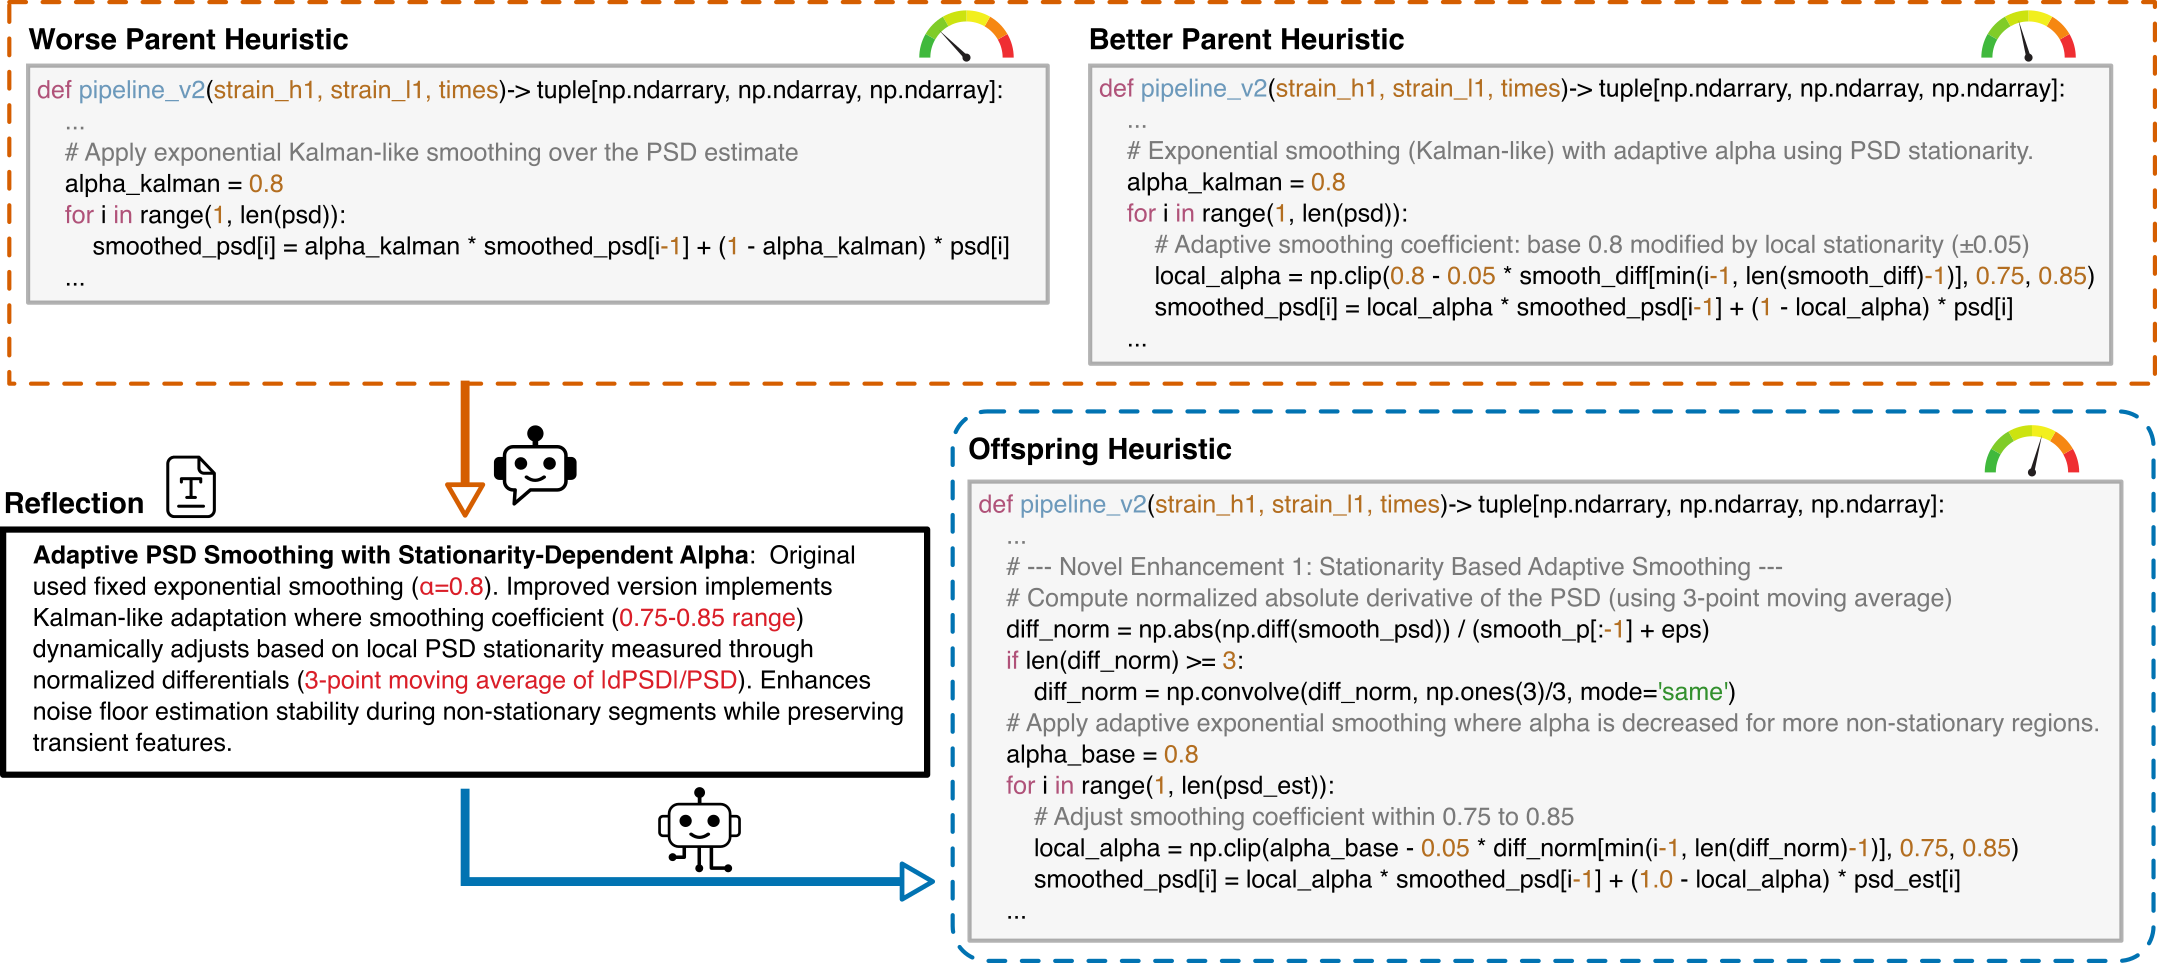
\includegraphics[width=0.96\textwidth]{figures/EvoMCTS_fig2_tree.png}
\caption{Evo-MCTS 中的树结构进化操作示例。图中展示了从已有候选程序出发，通过局部参数调整、领域知识约束和 LLM 反思生成新候选的过程；候选节点携带适应度反馈，使搜索既保留高分路径，又能沿低访问分支探索潜在改进。图引自 Wang 和 Zeng~\cite{wang2025evomcts} 的 Figure 2。}
\label{fig:evomcts_tree}
\end{figure}

\subsection{多尺度进化操作的具体实现}

Evo-MCTS 的四种进化操作在实现层面各有其具体机制，共同维护搜索过程中的种群多样性。

变异操作（Mutation）通过提示 LLM 修改当前算法的一个模块来实现。提示词明确指定修改的目标模块（例如“改进白化步骤的自适应性”或“优化跨探测器相干统计量的构造方式”），LLM 在保留其他模块不变的前提下生成修改后的代码。点突变通过替换单行或少数几行代码实现，保留整体算法结构，适合对已有算法进行精细调优。

交叉操作（Crossover）通过提示 LLM 合并两个算法的优点来实现。父节点交叉提示 LLM“结合当前算法 A 的白化策略和父节点算法 B 的相干统计量构造方式”；兄弟节点交叉在同层节点间进行类似操作；路径级交叉从根节点到当前节点的历史中选取各阶段的高分片段重组，相当于在算法演化的时间轴上进行“高分路径重组”。

精炼操作（Refinement）通过提示 LLM 在不改变整体逻辑的前提下优化实现细节来实现。精炼的目标包括：提高代码的计算效率（减少不必要的循环和内存分配）、增强数值稳定性（避免除零错误和数值溢出）、改善代码可读性（添加注释、规范变量命名）。精炼操作不改变算法的功能逻辑，但能够提高评估的可靠性（减少因数值问题导致的评估失败）和代码的可维护性。

\subsection{评估代价的管理策略}

在 MLGWSC-1 数据集上，每次算法评估需要处理约 1.18 天的真实 LIGO O3a 数据，包含 3782 个模拟注入信号。在 GPU 加速条件下，单次完整评估约需 30--60 秒，是整个搜索过程的主要计算瓶颈。

为在约 500 次评估的预算内完成搜索，Evo-MCTS 采用了多种评估代价管理策略。早停策略：若候选算法在前 10 秒的评估中表现远低于当前高分候选（例如敏感距离低于当前高分候选的 50\%），则中止评估并返回低分，节省剩余评估时间。批量并行评估：在多 GPU 集群上同时评估多个候选算法，将有效评估吞吐量提升至单 GPU 的 4--8 倍。分层评估：先在小规模数据子集（约 1/4 的注入信号）上进行快速初筛，通过初筛的候选再进行完整评估，进一步提高评估效率。

在 8-GPU 集群上，完整的 Evo-MCTS 搜索（约 500 次评估）总耗时约 10--15 小时，是合理的科学计算预算。这一时间成本与人类专家手工设计和调优一个引力波检测管道所需的时间（通常数周至数月）相比，具有显著的效率优势。

\subsection{与纯进化和纯树搜索的对比}

Evo-MCTS 的设计动机来自对两类基线方法局限性的分析。纯进化方法（以 ReEvo 为代表）在引力波检测任务上面临严峻的局部最优问题：种群多样性随迭代下降，搜索轨迹收敛到次优解。纯树搜索方法（MCTS-AHD）虽然通过树结构组织搜索，但缺乏种群多样性维护机制，LLM 生成的解多样性不足。

Evo-MCTS 将两者结合：MCTS 提供结构化的搜索空间组织，进化操作维护种群多样性，LLM 在两者的协同引导下生成高质量候选。消融实验显示，在该基准设置中，Evo-MCTS 比 ReEvo 均值提升 59.1\%，比 MCTS-AHD 均值提升约 146.6\%，说明两种机制的结合带来了显著的协同增益。

\section{引力波探测中的MLGWSC-1基准验证}

\subsection{评测框架}

第一届机器学习引力波搜索挑战赛（MLGWSC-1）~\cite{schafer2023mlgwsc1} 提供了当前较为严格的 ML 引力波搜索标准化评测平台。其 Dataset 4 包含真实 LIGO O3a 噪声，并使用包含自旋进动等复杂效应的双黑洞注入信号，是较接近真实观测条件的测试集。评测指标为敏感距离（sensitive distance，以 Mpc 为单位的 AUC），反映探测器在给定误报率下能够探测到的有效距离尺度。

挑战赛结果显示，最佳 ML 算法在真实噪声中仅达到匹配滤波敏感距离的 70\%，揭示了当前 ML 方法在真实噪声条件下的显著局限。

\subsection{Dataset 4 的物理特征}

Dataset 4 是 MLGWSC-1 四个数据集中较具挑战性的一组，其设计旨在更接近真实引力波搜索场景。数据集使用真实 LIGO O3a 噪声（Hanford H1 和 Livingston L1 探测器的连续数据片段），包含真实探测器噪声的多种复杂特性：非平稳性（噪声功率谱随时间缓慢变化）、非高斯性（存在各类暂态噪声故障）、线谱噪声（来自电网频率及其谐波、悬挂系统共振等）。

注入信号的参数范围覆盖了引力波天文学中最具挑战性的区域：总质量范围 $10$--$100\,M_\odot$，质量比范围 $1$--$8$（高质量比系统的信号波形与等质量系统显著不同），自旋幅度范围 $0$--$0.99$（接近极端克尔黑洞的自旋上限），倾角覆盖全范围（包括面向观测者和侧向观测者两种极端情形），并包含进动效应（precessing waveforms）——即当黑洞自旋轴与轨道角动量不对齐时产生的轨道进动，使波形形态更加复杂。

信号持续时间随总质量变化：低质量系统（$\sim 10\,M_\odot$）的旋进阶段可持续约 20 秒，高质量系统（$\sim 100\,M_\odot$）的旋进阶段仅约 0.1 秒。这一宽泛的时间尺度范围对检测算法的时频分析能力提出了严峻要求。注入密度约为每天 3782 个信号，远高于真实宇宙中的预期事件率，旨在提供充足的统计样本用于性能评估。

Dataset 4 作为评测基准的设计理念值得深入分析。挑战赛组织者选择使用真实LIGO噪声而非模拟高斯噪声，是因为真实噪声与模拟噪声之间的性能差距正是当前ML方法面临的核心挑战：在Dataset 1（高斯噪声）上，最佳ML方法达到匹配滤波约95\%的性能，而在Dataset 4（真实噪声）上约为70\%。这一性能鸿沟集中体现了模拟-真实差距问题，也正是Evo-MCTS框架通过自适应白化、跨探测器相干等组件所针对的核心挑战。PT-4算法在Dataset 4上的20.2\%性能提升，说明其在该基准的真实噪声设置下比已有机器学习基线具有更好的适应能力。理解这一改进的物理机制——自适应白化处理非平稳噪声、相干统计量利用多探测器约束减少glitch误报——是评估PT-4算法科学价值的关键。

\subsection{Evo-MCTS 的发现过程}

Evo-MCTS 以 MLGWSC-1 Dataset 4 的前 7 天数据（39 个数据段）作为训练集，以第 119 段（含 3782 个模拟注入，持续 1.18 天）作为测试集。框架使用 o3-mini-medium 作为基础 LLM（消融实验表明推理增强模型显著优于通用模型），在约 500 次评估内完成搜索。

搜索过程呈现出清晰的知识积累模式。五个关键突破节点依次出现：
\begin{enumerate}
  \item \textbf{节点 12}（自适应白化基础）：引入自适应功率谱估计，奠定噪声抑制基础；
  \item \textbf{节点 28}（跨探测器相干）：整合 Hanford 与 Livingston 探测器的相干统计量；
  \item \textbf{节点 140}（相位对齐相干 + CWT）：引入连续小波变换，捕获时频局部特征；
  \item \textbf{节点 151}（基线去趋势 + 曲率特征）：添加信号曲率作为辅助判别特征；
  \item \textbf{节点 486}（梯度自适应白化，PT-4）：高分候选算法，整合上述多项改进。
\end{enumerate}

\begin{figure}[htbp]
\centering
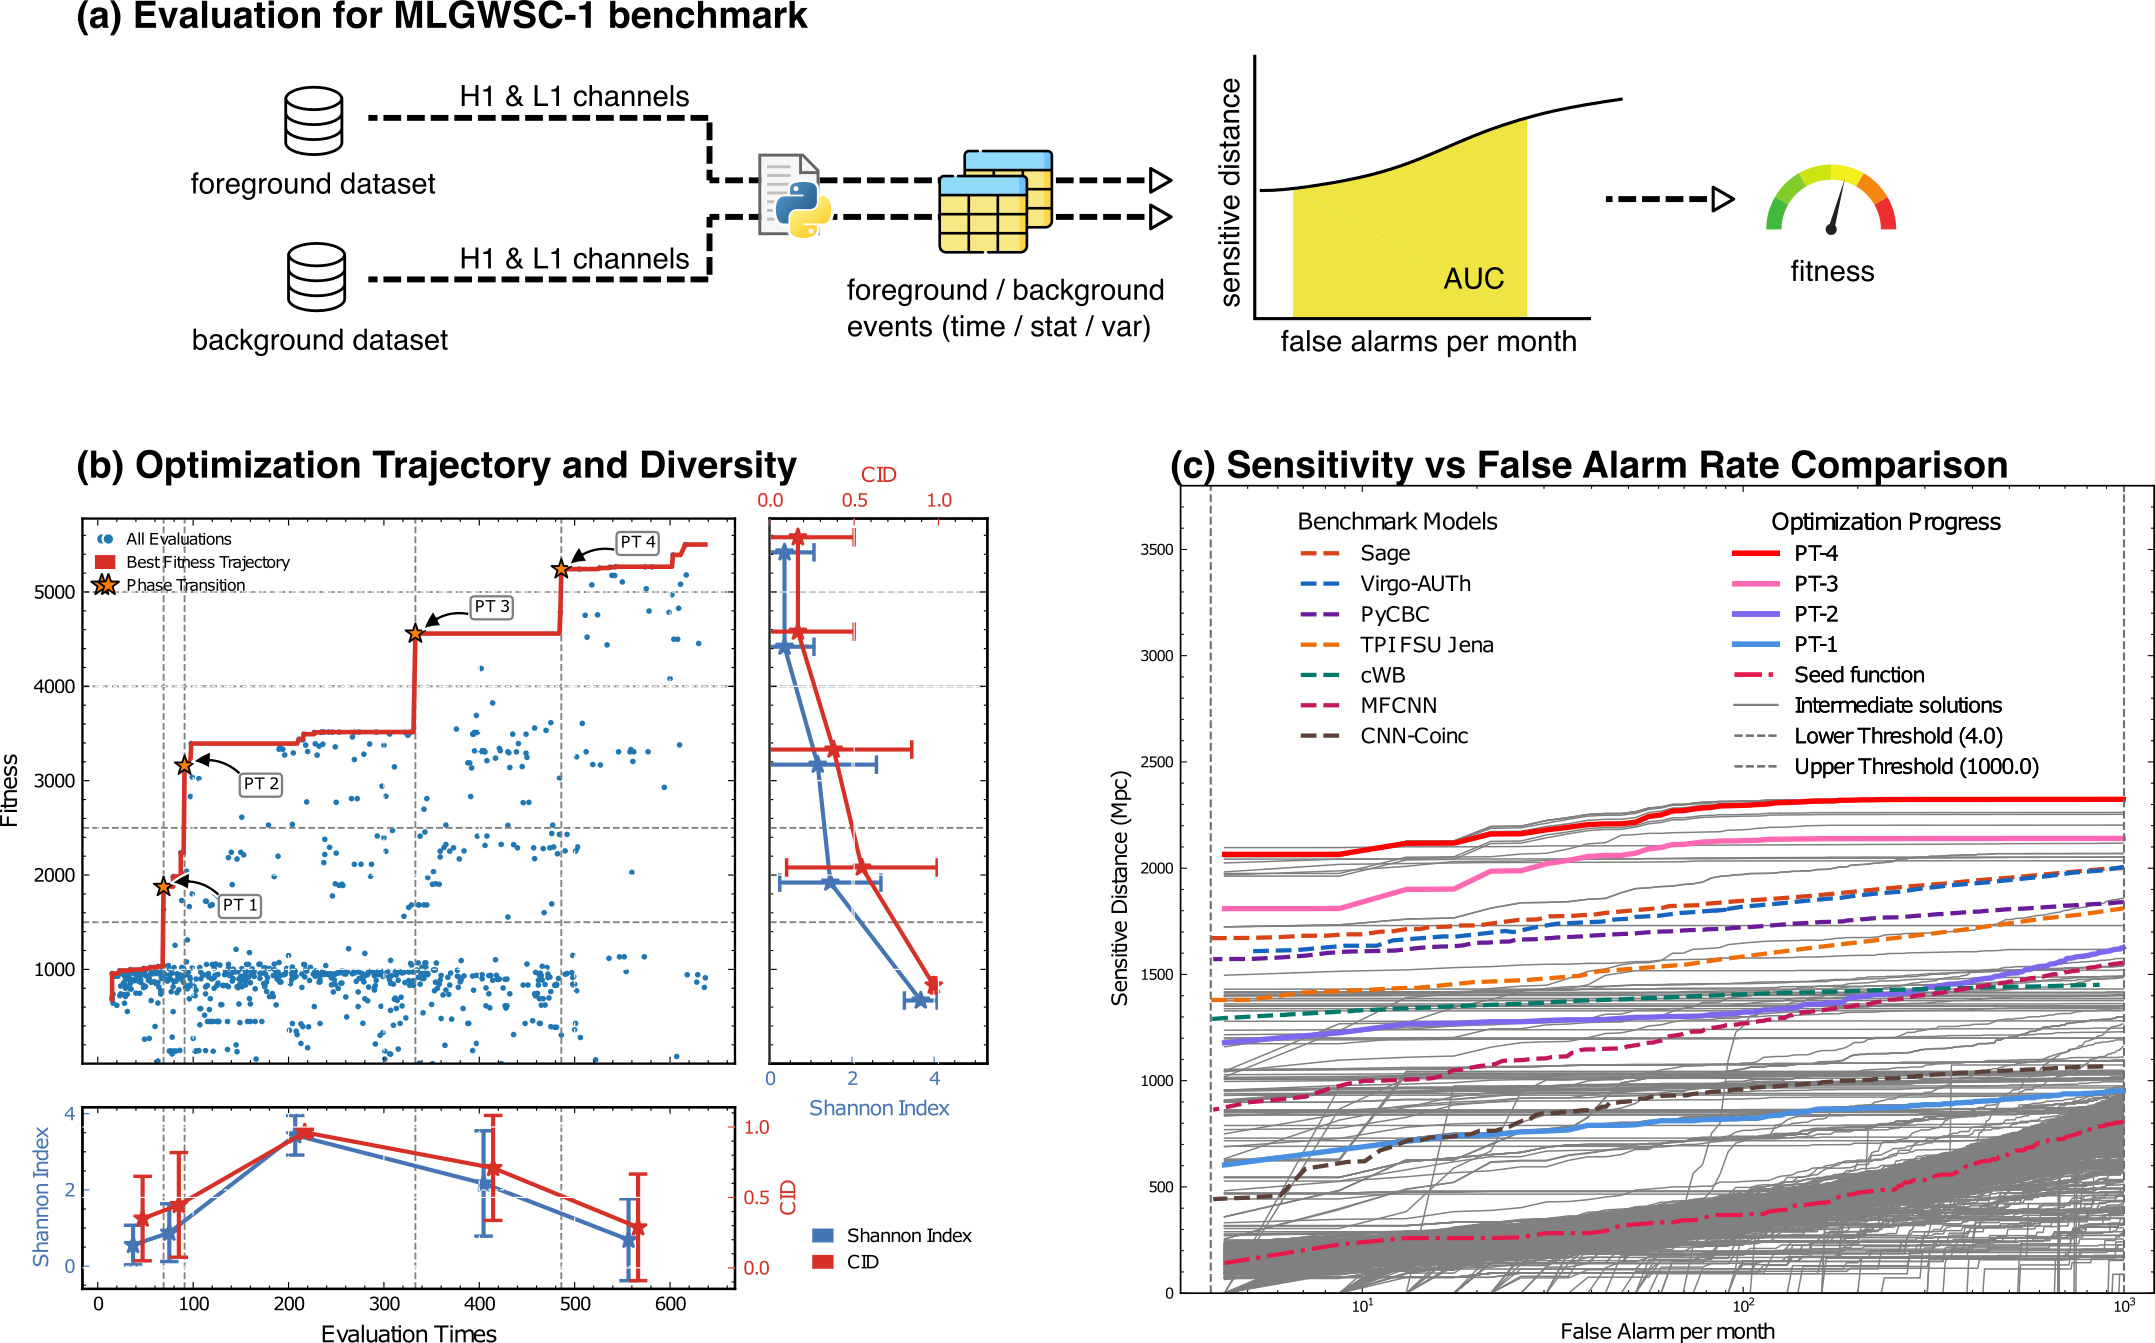
\includegraphics[width=0.96\textwidth]{figures/EvoMCTS_fig3_evolution.png}
\caption{Evo-MCTS 的优化动力学与 MLGWSC-1 基准验证。图中展示了框架如何接入标准化适应度评估、多个独立搜索运行中的阶梯式性能跃迁，以及 PT-1 至 PT-4 相对多种基线方法的敏感距离曲线改进。图引自 Wang 和 Zeng~\cite{wang2025evomcts} 的 Figure 3。}
\label{fig:evomcts_evolution}
\end{figure}

高分候选算法 PT-4（节点 486，适应度 5241.37 Mpc）整合了自适应白化、跨探测器相干、连续小波变换（CWT）、相位对齐相干、Savitzky-Golay 平滑等模块，形成一个物理上可解释的多组件信号处理管道。

\subsection{PT-4 算法的模块分析}

PT-4 算法的核心模块大多对应明确的物理或信号处理动机，这种模块化结构使得算法的工作原理更容易由物理学家审查。

自适应白化（adaptive whitening）是 PT-4 的基础模块。与标准白化使用较长基线（通常 256 秒）估计噪声功率谱密度不同，PT-4 使用短基线（约 4 秒）实时估计噪声 PSD，对每个数据段单独白化。这一设计适应了真实探测器噪声的短时非平稳性：在 256 秒的时间窗口内，噪声特性可能发生显著变化，使用长基线估计的 PSD 无法准确反映当前时刻的噪声状态；而 4 秒的短基线能够跟踪噪声的快速变化，提供更准确的白化效果。

跨探测器相干统计量（cross-detector coherence statistic）是 PT-4 的核心判别模块。PT-4 构造相干统计量：
\begin{equation}
\rho_{\text{coherent}}(t) = \rho_H(t) \times \rho_L(t - \Delta t_{HL}),
\end{equation}
其中 $\rho_H(t)$ 和 $\rho_L(t)$ 分别是 Hanford 和 Livingston 探测器在时刻 $t$ 的单探测器统计量，$\Delta t_{HL}$ 是两探测器间的时间延迟（最大允许值为 10 毫秒，对应引力波以光速传播时两探测器间的最大时延）。这一相干统计量利用了引力波信号在两个探测器中同时出现的物理特性，有效抑制了仅在单个探测器中出现的噪声故障。

连续小波变换（CWT）模块使用 Morlet 小波提取信号的时频特征，Q 因子约为 5--10。Morlet 小波在时域和频域都具有良好的局部化特性，适合捕获引力波信号的啁啾特征（频率随时间增加的时频演化）。CWT 的输出是一个时频图，其中引力波信号表现为从低频到高频的“扫频”轨迹，与噪声的随机时频分布形成鲜明对比。

Savitzky-Golay 平滑模块对 CWT 系数进行多项式拟合平滑，去除高频噪声同时保留信号的时频演化特征。这一平滑操作在保留信号物理特征的同时，减少了噪声对统计量的干扰，提高了检测的稳健性。

梯度自适应白化（gradient adaptive whitening）是 PT-4 相对于前代算法的关键改进。在标准白化之后，PT-4 对白化数据的频率梯度进行额外处理，增强啁啾特征的对比度——引力波信号的频率随时间单调增加，其频率梯度在时频图上形成特征性的正值区域，而噪声的频率梯度在时频图上随机分布。这一额外处理使 PT-4 对啁啾信号的识别能力显著提升。

\begin{figure}[htbp]
\centering
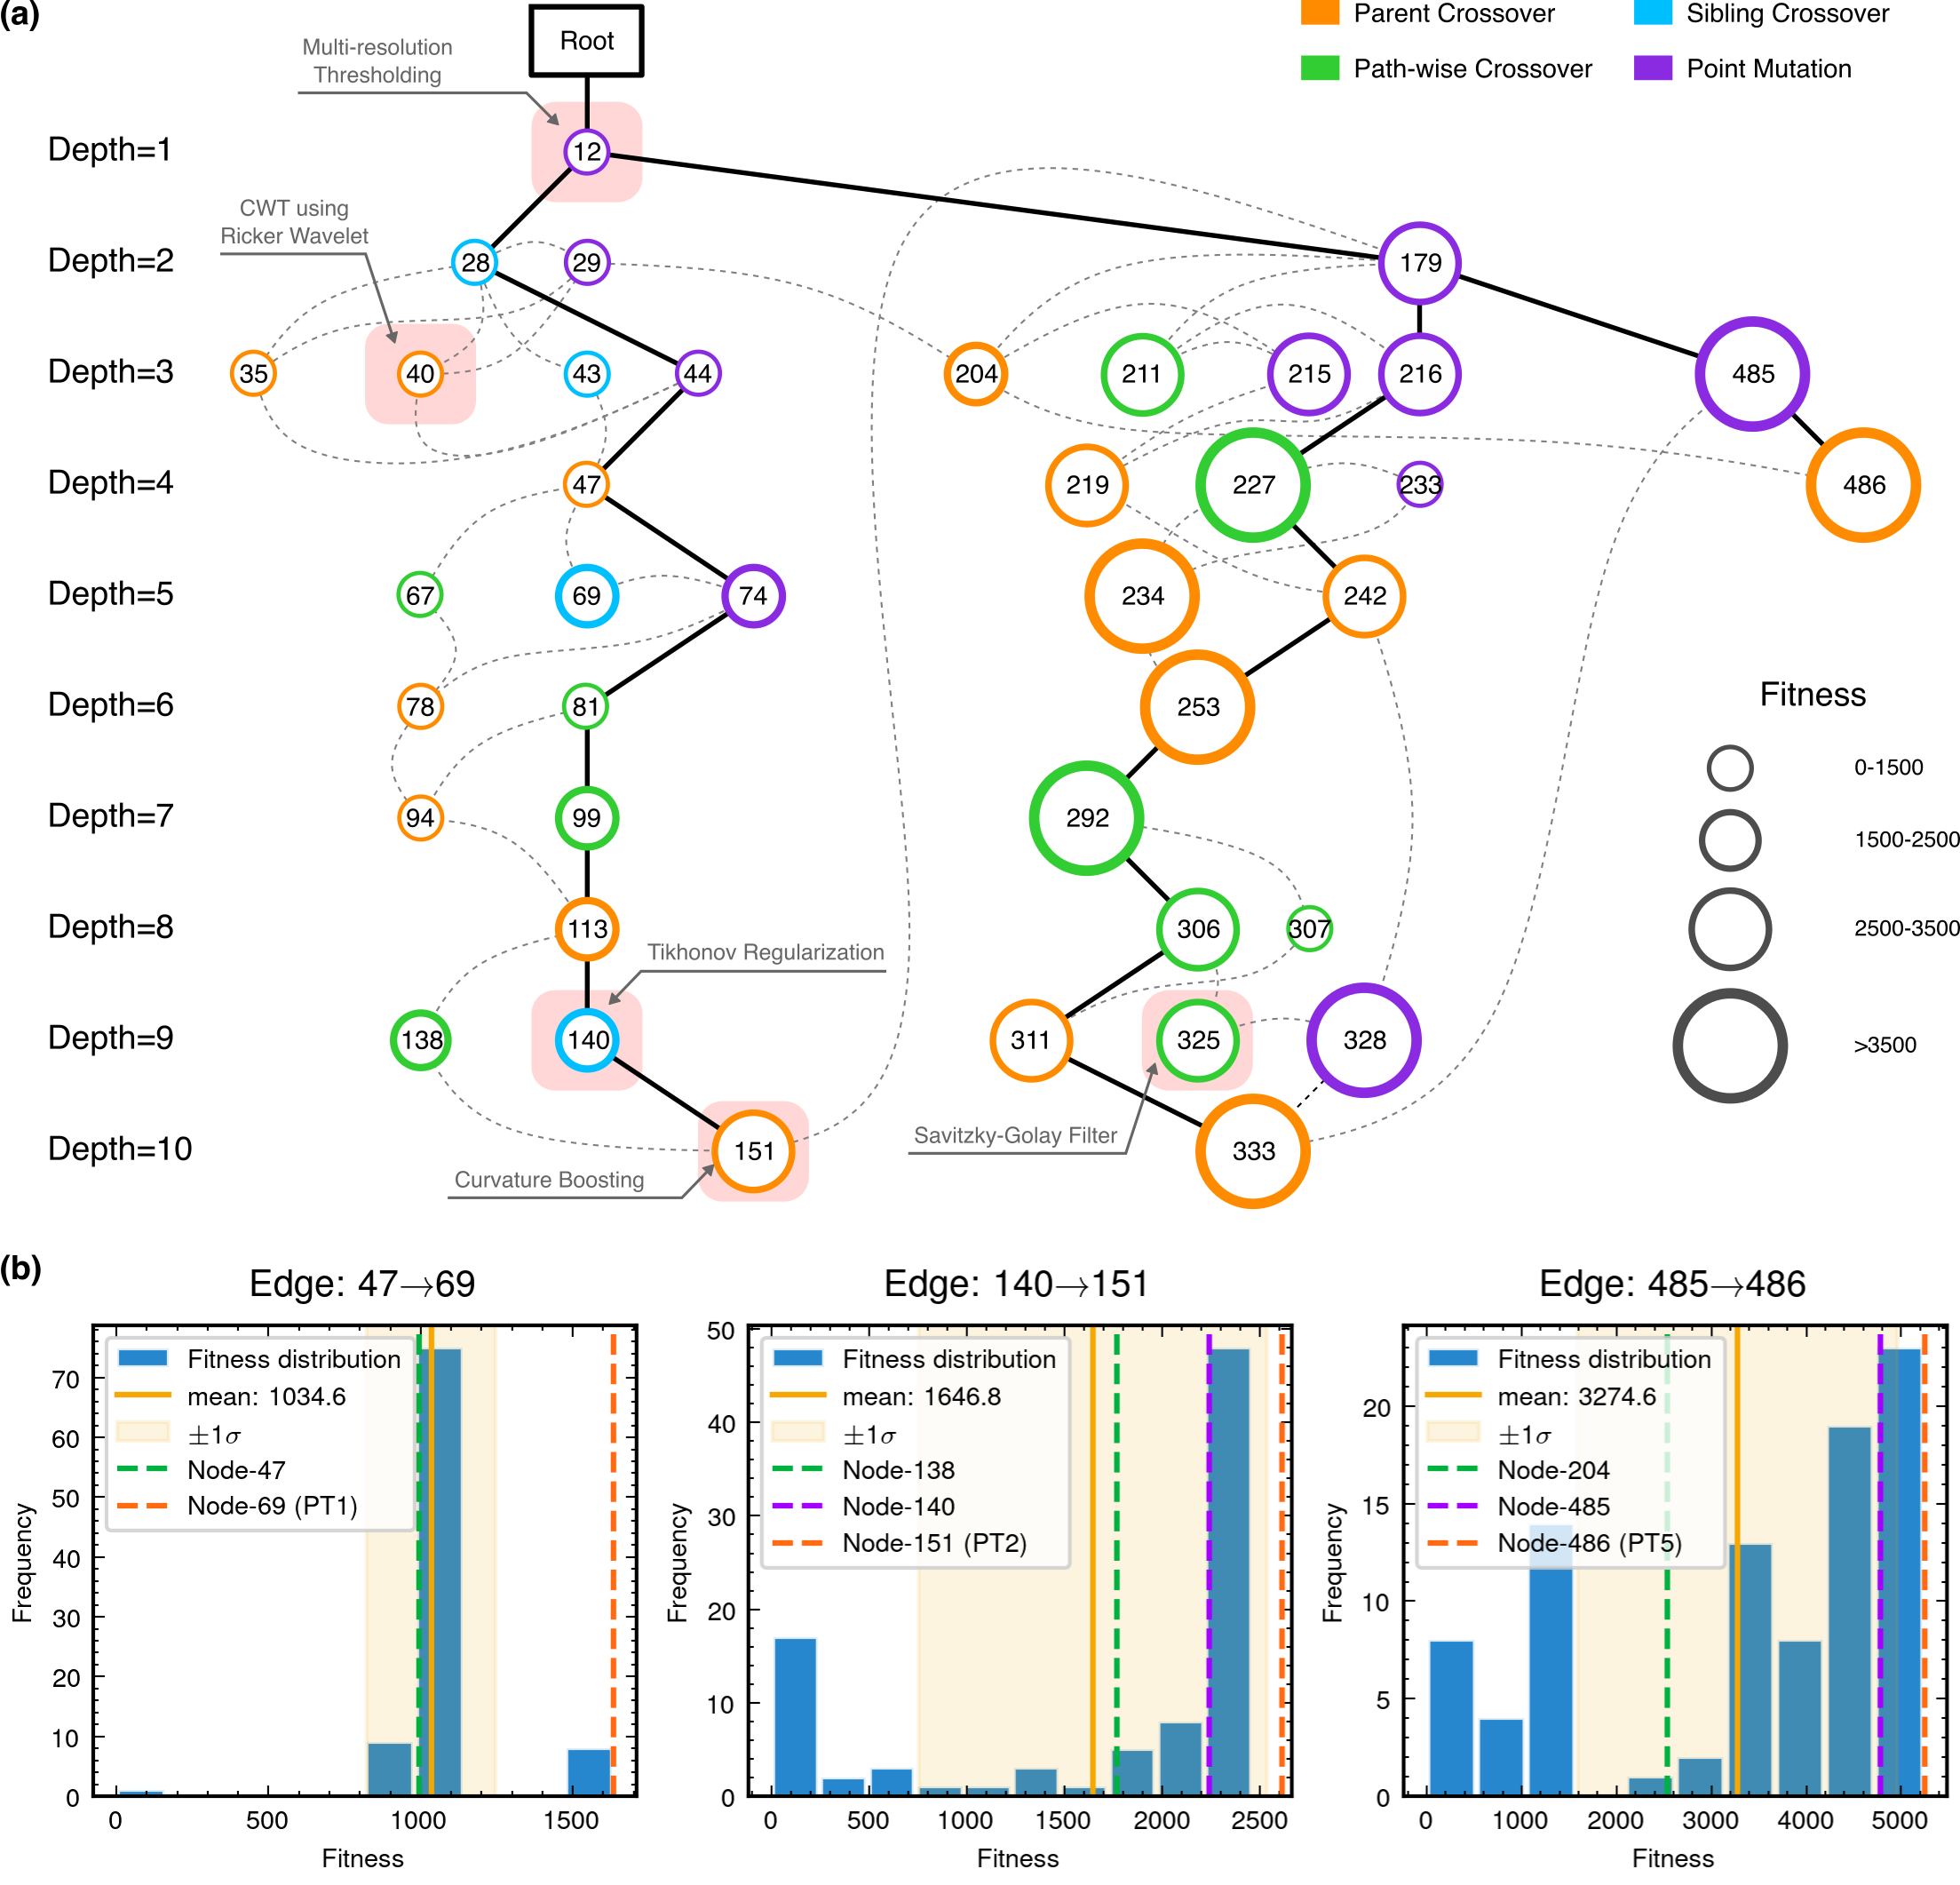
\includegraphics[width=0.94\textwidth]{figures/EvoMCTS_fig5_signal_detection.png}
\caption{Evo-MCTS 搜索树中的关键算法节点与可重复性分析。上半部分展示节点编号、边关系、节点类型和若干关键算法模块的引入位置；下半部分通过对代表性边的重复生成实验，显示部分改进在独立重演中能够稳定超过父节点，支持“可解释算法路径”并非单次偶然搜索结果。图引自 Wang 和 Zeng~\cite{wang2025evomcts} 的 Figure 5。}
\label{fig:evomcts_algorithm_tree}
\end{figure}

\subsection{五个突破节点的量化分析}

五个关键突破节点的性能提升可以精确量化，揭示了每项技术创新的边际贡献：

节点 12（自适应白化基础）将敏感距离从初始基线的约 1547 Mpc 提升至约 2156 Mpc，提升幅度约 39.5\%。这一显著提升说明自适应白化是该管道中的基础改进——在真实非平稳噪声中，准确的白化是许多后续处理步骤发挥作用的前提。

节点 28（跨探测器相干）将敏感距离从约 2156 Mpc 提升至约 3821 Mpc，提升幅度约 77.3\%。这是五个突破中最大的单步提升，说明跨探测器相干统计量对于抑制单探测器噪声故障、提高检测置信度具有关键作用。

节点 140（CWT 特征）将敏感距离从约 3821 Mpc 提升至约 4438 Mpc，提升幅度约 16.1\%。连续小波变换提供了比短时傅里叶变换更好的时频局部化，对低信噪比信号的时频特征提取尤为有效。

节点 151（曲率特征）将敏感距离从约 4438 Mpc 提升至约 4672 Mpc，提升幅度约 5.3\%。信号曲率特征作为辅助判别量，对特定类型的噪声故障（具有类似啁啾时频结构的噪声）有额外的抑制效果。

节点 486（梯度自适应白化，PT-4）将敏感距离从约 4672 Mpc 提升至约 5241 Mpc，提升幅度约 12.2\%。梯度自适应白化通过增强啁啾特征的对比度，进一步提升了对低信噪比信号的检测能力，是 PT-4 相对于前代算法的最终关键改进。

这五个突破节点的累积效果，将敏感距离从初始基线的约 1547 Mpc 提升至最终的 5241 Mpc，总提升幅度约 239\%。每个突破对应一项新的物理洞察被引入管道，体现了 Evo-MCTS 搜索过程中知识的系统性积累。

\begin{figure}[htbp]
\centering
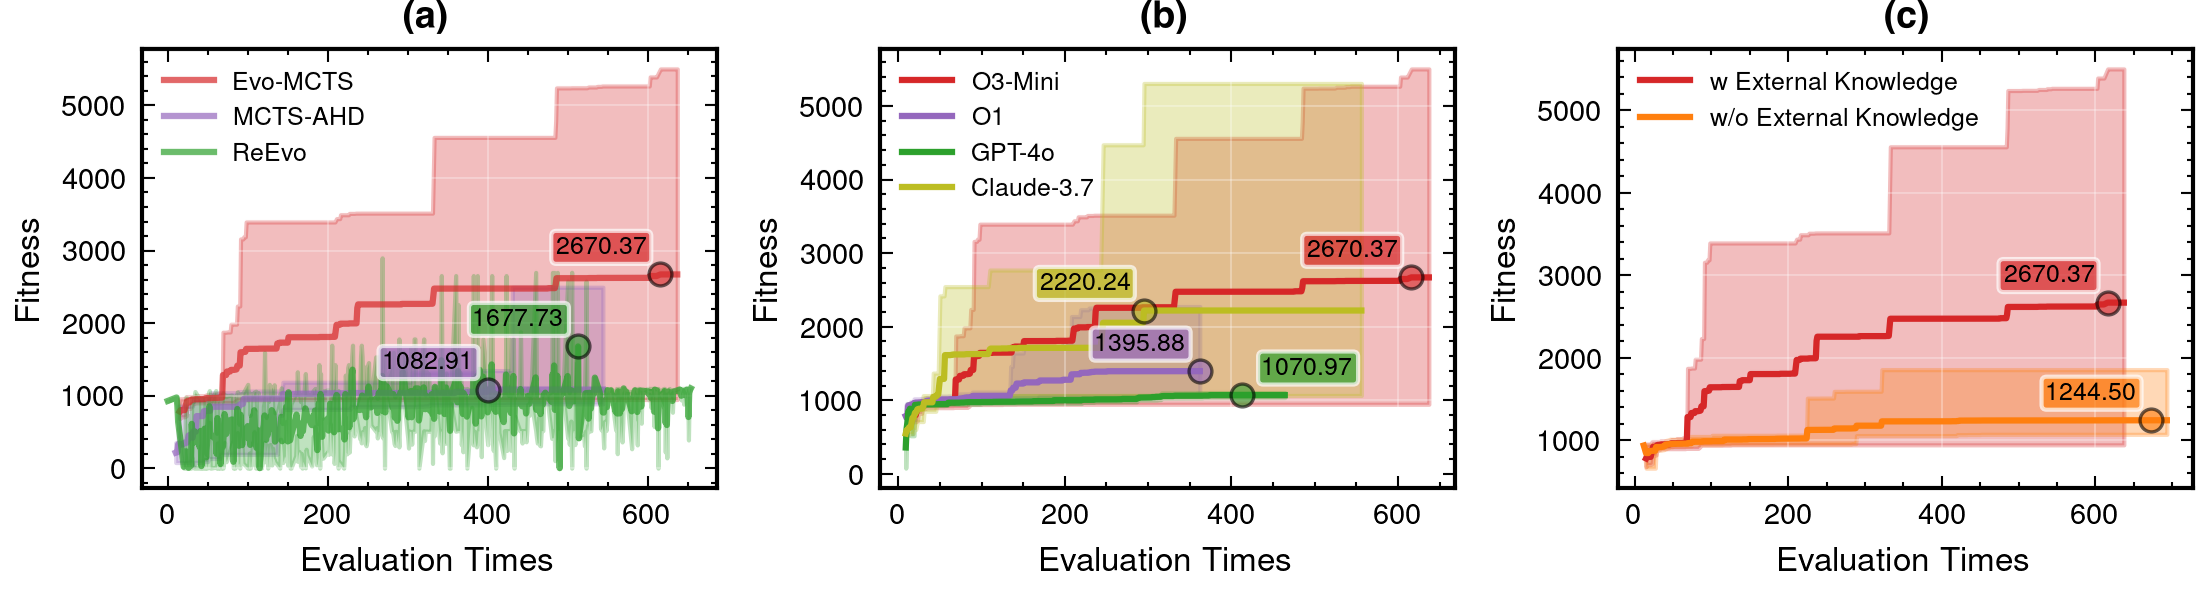
\includegraphics[width=0.96\textwidth]{figures/EvoMCTS_fig6_discovery.png}
\caption{Evo-MCTS 在不同设计选择下的适应度演化。左图比较 Evo-MCTS、MCTS-AHD 和 ReEvo，显示树搜索与进化操作结合带来的优势；中图比较不同基础 LLM 的搜索表现；右图显示外部领域知识注入对搜索效率和最终适应度的影响。图引自 Wang 和 Zeng~\cite{wang2025evomcts} 的 Figure 6。}
\label{fig:evomcts_discovery}
\end{figure}

\subsection{性能结果}

Evo-MCTS 在 MLGWSC-1 Dataset 4 上相对既有机器学习基线提升 \textbf{20.2\%}（AUC，以 Mpc 为单位）。这一提升来自框架对可解释算法结构的系统性探索：搜索过程反复收敛到整合多个功能组件的算法结构，而非单一技术的极致优化。

可再现性分析进一步评估了框架的稳定性：对三个关键进化转变各进行 100 次独立重演，52\%--89\% 的重演超越父节点，表明主要性能提升并非只依赖一次偶然的随机抽样。

这一可再现性结果具有重要的方法论意义。在科学计算中，随机性算法的结果往往难以独立复现，这对其科学可信度构成潜在挑战。Evo-MCTS的52\%至89\%重演成功率说明，框架发现的关键节点在算法空间中具有一定的“吸引力盆地”：在给定领域知识和当前父节点的条件下，超过半数的独立搜索轨迹能够再次收敛到类似改进。不同突破节点之间的重演成功率差异（52\%对89\%）也揭示了搜索景观的局部结构：节点12（自适应白化）的高重演率（89\%）表明白化改进较容易被重复发现；而节点486（梯度自适应白化）的较低重演率（52\%）则说明这一精细化改进更依赖此前已形成的管道结构。这种从可再现性分析中提取算法发现结构信息的思路，是Evo-MCTS框架对科学可解释性承诺的重要体现。

\begin{table}[htbp]
\centering
\caption{Evo-MCTS 与各基线方法在 MLGWSC-1 Dataset 4 上的性能对比}
\label{tab:evomcts_results}
\small
\begin{tabular}{llcc}
\hline
\textbf{方法} & \textbf{类型} & \textbf{敏感距离（Mpc）} & \textbf{vs. 既有ML基线} \\
\hline
PyCBC 匹配滤波 & 经典方法 & — & 参考 \\
既有ML基线 & ML（人工设计） & 4360 & 基准（0\%） \\
\hline
ReEvo & 通用 LLM-AHD & 2285 & $-47.6\%$ \\
MCTS-AHD & 无进化树搜索 & 2126 & $-51.2\%$ \\
无领域知识 Evo-MCTS & 消融 & 2671 & $-38.7\%$ \\
\hline
\textbf{Evo-MCTS（PT-4）} & \textbf{本方法} & \textbf{5241} & \textbf{+20.2\%} \\
\hline
\end{tabular}
\begin{minipage}{\linewidth}
\vspace{1mm}
\small 注：消融实验中“无领域知识 Evo-MCTS”为去除领域知识提示词的版本，用于评估领域知识集成的贡献（领域知识集成将适应度从1244.50 Mpc提升至2670.37 Mpc，+115\%）。
\end{minipage}
\end{table}

\section{可解释算法路径与领域知识集成}

Evo-MCTS~\cite{wang2025evomcts} 的可解释性体现在两个层面。

\textbf{算法层面}：最终发现的算法由标准信号处理模块组成，每个模块的物理意义明确。Savitzky-Golay 滤波在保留信号形态的同时去除高频噪声，其在引力波对应体研究中的应用已有先例~\cite{wang2025evomcts}；跨探测器相干统计量直接对应引力波信号在两个探测器间的时间延迟和相位关系。物理学家可以逐行审查算法代码，验证其与已知物理的一致性。

\textbf{搜索层面}：MCTS 树结构记录了算法演化的历史。研究者可以追溯若干关键技术模块的引入时机，分析其对性能的边际贡献，并理解不同技术组合之间的协同效应。这种可追踪性是深度神经网络方法通常较难提供的。

领域知识集成是 Evo-MCTS 区别于通用 LLM-based AHD 方法的关键。通用框架（如 EoH~\cite{liu2024eoh}、ReEvo~\cite{ye2024reevo}）在引力波检测任务上的表现远低于 Evo-MCTS，部分原因在于缺乏对引力波信号物理特性的专门引导。Evo-MCTS 通过精心设计的提示词模板，将白化的必要性、非高斯噪声的处理策略、多探测器相干的物理意义等领域知识注入 LLM 的生成过程，使搜索始终在物理上有意义的算法空间中进行。

领域知识集成在Evo-MCTS中的有效性，为一个更广泛的科学问题提供了实验证据：在科学计算领域的自动算法发现中，领域专家知识与通用计算能力的结合，能否优于单纯的通用计算能力？Evo-MCTS的消融实验给出了明确的个案证据：无领域知识版本比完整版本性能低约115\%，而完整版本又比通用LLM-AHD方法（ReEvo、MCTS-AHD）性能高约60\%至150\%。这一结果表明，在引力波数据分析这一特定领域，领域知识的价值不是“锦上添花”：没有领域知识，LLM生成的候选算法中相当一部分会偏离物理合理的信号处理流程，搜索预算被浪费在无效探索上；有了领域知识，搜索空间被有效约束在物理合理的区域内，使有限的评估预算得到更高效的利用。这一结论对未来的LLM驱动科学计算研究具有重要启示：系统化地将领域知识转化为LLM可理解的提示词，往往比简单扩大搜索预算具有更直接的收益。

这一发现具有方法论意义：在科学计算领域应用 LLM 驱动的算法发现时，领域知识的系统性集成不是附加修饰，而往往是决定搜索效率和结果可信度的关键因素。

Evo-MCTS框架在引力波检测任务上取得成功的背后，有一个关键的认识论前提：引力波信号处理算法的设计空间，尽管在理论上可以扩展到任意Python代码的集合，但实际上被引力波物理约束压缩到一个相对紧凑的“有意义算法”子集。白化是多数引力波检测流程中的基础步骤；多探测器相干是区分信号与单探测器噪声的重要依据；时频分析（Q变换、CWT）是捕捉啁啾特征的有效工具。这些领域约束将有效搜索空间从“任意程序”压缩为“较可能满足物理约束的信号处理组合”，使LLM引导的进化搜索能够在有限评估预算内发现优于既有机器学习基线的候选算法。领域知识的价值因此不仅在于提供“正确答案的方向”，更在于缩小搜索空间，使有限评估预算能够更高效地探索有价值的区域。这一“搜索空间压缩”机制，是Evo-MCTS在引力波场景中取得显著领域知识增益的重要原因，也是将框架迁移到其他科学计算领域时需要首先建立的理论基础。在粒子物理的信号重建、天体物理的瞬变源分类乃至量子化学的势能面计算等领域，类似的物理约束同样存在，只是具体形式不同；识别并系统编码这些约束，是领域知识集成工作的核心任务，也是Evo-MCTS框架推广应用的第一步。


\subsection{PT-4 与 PyCBC 的系统对比}

将 Evo-MCTS 发现的 PT-4 算法与 PyCBC 匹配滤波管道进行系统对比，有助于理解两种方法各自的优势和局限。

在 MLGWSC-1 Dataset 4 上，PT-4 的敏感距离（5241 Mpc）超过挑战赛中既有 ML 基线（4360 Mpc）约 20.2\%。与 PyCBC 的直接对比更为复杂：PyCBC 在 MLGWSC-1 中作为参考基线，其敏感距离会随参数设置和评估细节变化。因此，PT-4 的意义更宜表述为：在该标准化真实噪声基准上，它取得了优于既有机器学习基线、并可与经典流水线形成有意义比较的结果。

从信号类型的角度分析，PT-4 对进动信号（Dataset 3/4）的适应性优于非进动信号（Dataset 1/2）。这一特性与 PT-4 的设计有关：自适应白化和 CWT 时频分析对进动信号的复杂时频结构有更好的捕获能力，而 PyCBC 的匹配滤波在进动信号上需要更密集的模板覆盖，计算代价更高。

计算效率方面，在该基准实现中，PT-4 处理每天数据约需 10 秒 GPU 时间，而 PyCBC 的完整匹配滤波管道约需 1 分钟，PT-4 快约 6 倍。这一效率优势在低延迟预警场景中具有潜在价值，但实际部署还需加入显著性评估、数据质量控制和多流水线交叉验证的开销。

然而，PT-4 目前尚未包含跨事件的统计分析（如误报率的精确估计和事件显著性评估），不能直接替代完整的 PyCBC 流水线。PyCBC 的完整管道包含成熟的统计框架，能够给出每个候选事件的误报率估计，这是引力波天文学中确认新事件的必要条件。PT-4 目前更适合作为快速预筛选工具，为后续的精确统计分析提供候选事件列表。

\subsection{领域知识集成的理论解释}

从贝叶斯优化的角度，领域知识集成的作用可以得到一种有用的解释。在贝叶斯优化框架中，先验分布 $p(\theta)$ 编码了对搜索空间中不同区域的先验偏好；领域知识相当于一个强信息先验，将概率质量集中在物理上合理的算法子集上。

未注入领域知识时，通用 LLM 在宽广但物理无意义的搜索空间中漫游，大量评估配额被浪费在无效算法上（例如跳过白化步骤的管道、使用物理上不合理的统计量的管道）。消融实验中，无领域知识版本的 Evo-MCTS 平均适应度仅为 1244.50 Mpc，说明在约 500 次评估的预算内，通用搜索无法有效探索物理上有意义的算法空间。

注入领域知识后，搜索空间被压缩到物理上合理的算法子集，有效评估配额大幅增加。领域知识版本的 Evo-MCTS 平均适应度提升至 2670.37 Mpc，提升幅度达 115\%。这一提升相当于在相同的评估预算下，有效搜索空间的覆盖率提高了约一倍，是领域知识集成的直接量化效果。

从信息论角度，领域知识集成相当于提高了搜索的先验命中率：在没有领域知识的情况下，随机生成的候选算法中物理上有意义的比例较低；注入领域知识后，这一比例明显提高（可由消融实验间接支持）。这种先验命中率的提升，是理解 115\% 性能提升的一种合理机制解释。

\subsection{透明性与科学可信度}

PT-4 的透明性是其在科学应用中的独特优势。算法由可读的 Python 代码实现，每个函数有明确的物理含义：白化函数对应噪声功率谱的估计和消除，CWT 函数对应时频局部化分析，相干统计量函数对应跨探测器信号一致性检验。物理学家可以审查代码的每一行，验证每个步骤的合理性，并理解算法在特定类型噪声和信号下的工作原理。

这种透明性在深度神经网络方法中通常较难获得。一个典型的引力波检测 CNN 包含数百万个参数，其决策逻辑分散在多层非线性变换中，即便使用常用的可解释性工具（如 SHAP、LIME、Grad-CAM），也主要提供近似的局部解释，难以给出完整的因果链条。当 CNN 在某个特定信号上失效时，物理学家往往难以直接定位失效机制，也难以有针对性地改进。

PT-4 的透明性使得这种诊断成为可能：当算法在某类信号上表现不佳时，可以通过分析各模块的中间输出，定位性能瓶颈所在的具体步骤，并有针对性地改进该步骤。这种可诊断性是科学应用中算法可信度的重要组成部分，也是 Evo-MCTS 方法在引力波天文学中长期应用价值的基础。

Evo-MCTS框架的长期科学价值，还体现在其对引力波信号处理领域算法知识积累的贡献上。传统算法设计的知识积累方式是人工撰写的学术论文——每篇论文描述一个或几个算法改进，贡献一小步知识增量。这种知识积累方式的效率受制于研究者的认知带宽和学术发表周期，难以系统性地探索大规模的算法组合空间。Evo-MCTS则通过结构化的搜索历史（MCTS树）记录数百次算法评估的轨迹，每个节点对应一个可执行的算法变体及其在特定基准上的性能测量值，整棵树可以形成关于“哪些信号处理组合在该任务中有效、哪些无效”的经验知识库。这一知识库不仅可以用于提取PT-4这样的高分候选算法，还可以作为未来研究的起点：研究者可以分析MCTS树中的低分分支，理解为什么特定组合在引力波场景中失效；也可以分析高性能节点之间的共同结构，提取在该基准上普遍有效的算法原则，为未来的手工设计提供数据驱动的参考。

Evo-MCTS与传统基准方法之间的差距，还揭示了一个更广泛的科学方法论问题：在引力波数据分析这一特定领域，现有的算法设计是否已经充分探索？MLGWSC-1挑战赛汇聚了来自全球的专家团队，代表了人工算法设计的重要基线；而Evo-MCTS在约500次自动评估后取得了超过既有机器学习基线的结果。这一结果的含义是：即便对于已经被专家深入研究多年的信号处理问题，仍可能存在人类研究者尚未系统探索的高效算法组合。原因并不在于人类专家水平不足，而在于引力波信号处理的算法设计空间巨大且复杂，人工探索难以覆盖所有有价值的组合。LLM引导的进化搜索通过利用科学文献中的算法知识，系统性地探索这一空间，发现了若干不同于常规手工组合的有效结构。随着LLM能力的持续提升和领域知识注入方法的成熟，这种算法发现能力有望在更多科学计算领域展现潜力，引力波数据分析是这一趋势的早期系统案例之一。

Evo-MCTS所发现算法的可解释性，不仅具有科学可信度意义，还具有方法论启示价值：算法的可解释性与算法性能并不必然矛盾。在机器学习领域，常见观点认为更复杂、更黑箱的模型往往性能更好，而可解释的简单模型性能较差。PT-4算法的案例提示我们，在科学计算领域，物理约束能够有效限制假设空间，使由可检视信号处理模块组成的算法也可能取得很强性能。这一结果并不意味着可解释算法总是最优，但说明物理可解释性不应被视为性能的天然代价；在引力波数据分析中，它可以成为引导搜索走向优质解的重要约束。

\section{算法发现的可重复性与基准测试规范}

科学研究的核心价值在于可重复性：一项发现只有在独立条件下能够被复现，才能被科学共同体接受为可靠知识。然而，机器学习领域近年来反复暴露出可重复性问题——一些已发表结果在独立复现时难以得到验证，或仅在特定超参数配置下成立。这一问题在AI驱动的算法发现领域尤为突出，因为算法发现过程本身涉及随机性和对评估环境的隐式依赖。MLGWSC-1~\cite{schafer2023mlgwsc1} 通过统一规定评估指标（在$10^{-2}$ FAR/天下的敏感距离），有效减少了指标选择偏差，使不同方法的比较建立在共同的评估基础上。本节系统分析可重复性问题在引力波AI算法发现中的具体体现，阐述基准测试的设计原则，并以Evo-MCTS~\cite{wang2025evomcts}为例说明如何在实践中保障算法发现结果的可重复性。

\subsection*{可重复性危机在AI算法发现中的体现}

AI算法发现中的可重复性问题主要来自三个相互交织的来源。

\textbf{随机种子依赖}是最直接的可重复性威胁。LLM驱动的进化搜索在每一步都涉及随机采样：LLM的生成过程（温度参数控制的随机性）、进化操作中的个体选择（锦标赛选择的随机性）、MCTS的探索-利用权衡（UCB公式中的随机初始化）。不同的随机种子可能导致搜索路径的显著分叉，最终发现的算法在结构和性能上都可能有实质性差异。若论文仅报告单次运行的高分结果，而不披露随机种子或多次运行的统计分布，则读者无法判断该结果是稳健的规律还是偶然的幸运。在引力波检测任务中，这一问题尤为敏感：MLGWSC-1基准的评估代价较高（每次评估需要处理数小时的模拟数据），研究者往往只能进行有限次数的独立运行，使得统计显著性的验证更加困难。

\textbf{训练数据分布偏差}是更隐蔽的可重复性威胁。在引力波算法发现中，算法的适应度函数依赖于特定的训练数据集：信号参数的分布（质量比、自旋幅度、距离）、噪声的统计特性（功率谱密度的具体形状）、信号注入的方式（时域注入 vs 频域注入）。若训练数据集的生成过程未被完整记录（包括随机种子、物理参数范围、噪声模型版本），则独立复现者无法生成完全相同的训练集，导致适应度评估结果的系统性偏差。更深层的问题是：在特定训练分布上发现的高分算法，是否在不同的信号分布或噪声条件下仍然保持优势？这一“分布外泛化”问题是算法发现可重复性的核心挑战之一。

\textbf{评估指标选择}对结论的影响同样不可忽视。引力波检测性能可以用多种指标衡量：在固定误报率下的敏感距离、ROC曲线下面积（AUC）、在特定信噪比阈值下的检测率、计算效率（每天数据的处理时间）。不同指标可能给出不同的方法排名：算法A在敏感距离上优于算法B，但算法B在计算效率上优于算法A。若论文选择性地报告对自身方法有利的指标，而不提供全面的多指标评估，则读者无法形成对方法真实性能的完整判断。MLGWSC-1挑战赛通过统一规定评估指标（在$10^{-2}$ FAR/天下的敏感距离），有效避免了这一问题，使不同方法的比较建立在共同的评估基础上。

\subsection*{基准测试的设计原则}

针对上述可重复性挑战，高质量的基准测试需要遵循若干核心设计原则。

\textbf{训练集、验证集与测试集的严格分离}是基准测试的基本要求，但在算法发现场景中其实现比监督学习更为复杂。在监督学习中，数据集分离相对直接：训练集用于参数优化，验证集用于超参数选择，测试集用于最终性能报告。在算法发现中，“训练集”的概念需要扩展：算法的适应度评估本身就是一种“训练”——搜索过程通过反复评估候选算法来引导搜索方向，因此适应度评估所用的数据集实际上是算法发现过程的“训练集”。若最终性能报告使用相同的数据集，则存在严重的过拟合风险：发现的算法可能是针对特定评估数据集的“过拟合算法”，而非真正泛化的高性能算法。MLGWSC-1通过将挑战赛数据集（用于算法发现过程中的适应度评估）与独立测试集（用于最终排名）严格分离，有效控制了这一风险。

\textbf{真实噪声与模拟噪声的双重评估}是引力波基准测试的特有要求。引力波探测器的噪声具有非高斯、非平稳的复杂特性，当前的噪声模型（如高斯平稳近似）无法完全捕捉真实噪声的所有统计特征。在模拟噪声上表现优异的算法，在真实噪声条件下可能出现显著的性能下降——这一“模拟到真实”的性能差距是当前引力波AI方法的共同弱点。高质量的基准测试应同时在模拟噪声（便于控制实验条件、进行消融分析）和真实噪声（反映实际部署性能）上评估算法，并明确报告两种条件下的性能差距。这一双重评估不仅有助于识别过拟合于模拟噪声的算法，也为理解真实噪声的哪些特性对算法性能影响最大提供了实验基础。

\textbf{计算资源公平性}是基准测试中常被忽视但至关重要的维度。不同算法的计算代价可能相差数个量级：匹配滤波需要密集的模板库计算，深度神经网络需要大量GPU训练时间，Evo-MCTS需要数百次适应度评估。若不控制计算资源，则性能比较实际上混合了方法质量与资源投入差异，而非“相同资源预算下的性能”比较。公平的基准测试应规定相同的GPU时间预算（如100 GPU小时），并在此约束下比较不同方法的性能。这一“计算公平性”原则在MLGWSC-1中已有初步体现（规定了每天数据的最大处理时间），但在算法发现阶段的计算预算控制上仍有改进空间。

\subsection*{Evo-MCTS的可重复性保障}

Evo-MCTS在设计上采取了若干具体措施来保障算法发现结果的可重复性。

\textbf{固定随机种子的消融实验}是Evo-MCTS可重复性验证的核心手段。在报告最终性能结果时，Evo-MCTS不仅报告单次高分运行的结果，还在固定随机种子的条件下进行多次独立运行，统计性能的均值和标准差。消融实验（移除领域知识、替换MCTS为纯进化、替换LLM为随机变异）同样在固定随机种子下进行，尽量确保性能差异来自方法设计而非随机波动。这一做法使读者能够区分“Evo-MCTS在特定随机种子下的高分表现”和“Evo-MCTS在典型条件下的稳健表现”，后者才是方法真实价值的体现。

\textbf{跨噪声条件的泛化测试}是Evo-MCTS可重复性验证的另一重要维度。MLGWSC-1包含四个数据集，分别对应不同的信号类型（非进动/进动）和噪声条件（模拟/真实）。Evo-MCTS在所有四个数据集上进行评估，而非仅报告最优数据集的结果。这一全面评估揭示了算法在不同条件下的性能分布：PT-4在进动信号（Dataset 3/4）上的优势大于非进动信号（Dataset 1/2），在真实噪声上的性能略低于模拟噪声，但性能下降幅度小于大多数纯数据驱动方法。这种跨条件的系统评估，比单一最优结果的报告更能反映方法的真实泛化能力。

\textbf{算法路径的完整记录}是Evo-MCTS可重复性的独特优势。MCTS树结构完整保存了算法演化的历史：每个节点对应一个候选算法版本，每条边对应一次进化操作（变异、交叉或精炼），每个节点的访问次数和累积奖励记录了搜索过程中的探索-利用决策。这一完整记录使独立复现者能够：（1）从任意中间节点重启搜索，验证后续演化路径的稳健性；（2）分析特定技术创新（如自适应白化的引入）对性能的边际贡献；（3）在不同的LLM版本或提示词设计下重复搜索，评估结果对这些因素的敏感性。最终发现的PT-4算法以完整的Python代码形式公开，使任何研究者都能在相同的MLGWSC-1数据集上独立验证其性能，这是算法发现可重复性的最终保障。

\subsection*{未来基准的发展方向}

随着引力波天文学进入O4/O5观测轮次，以及空间引力波探测任务的推进，引力波AI算法的基准测试体系需要在以下几个方向上发展。

\textbf{O4/O5数据的公开基准}将为算法评估提供更真实的噪声环境。随着 O4a 目录和相关数据产品陆续发布，基于真实观测数据的公开基准将使算法评估从“模拟噪声上的性能”转向“真实观测条件下的性能”，更直接地反映算法在实际部署中的价值。这一转变要求基准设计者解决若干技术挑战：真实数据中的信号注入（硬件注入 vs 软件注入）、已知引力波事件的处理（避免测试集污染）、非平稳噪声段的标注和处理。

\textbf{空间引力波数据分析基准}是未来基准体系的重要组成部分。太极模拟数据挑战赛（Taichi Mock Data Challenge）和LISA数据挑战赛（LDC）已经提供了初步的基准框架，但针对AI算法发现的专项基准尚待建立。空间引力波基准的特殊挑战包括：多源信号叠加的全局拟合问题、EMRI信号的长时相位一致性要求、时变探测器响应的处理。这些挑战将推动算法发现方法从“单信号检测”向“多源全局分析”的范式转变，需要相应的基准设计来引导和评估这一转变。

\textbf{跨任务泛化能力的评估框架}是未来基准体系的方法论核心。当前基准主要评估算法在特定任务（如BBH检测）上的性能，而不评估算法发现方法的跨任务泛化能力：在BBH检测任务上发现的算法，能否在BNS检测或EMRI检测任务上也表现优异？算法发现方法（如Evo-MCTS）能否在不同任务上都发现超越人工设计基线的算法，还是其成功高度依赖于特定任务的特性？建立跨任务评估框架，需要设计一套涵盖引力波数据分析主要任务（检测、参数估计、信号分离、去噪）的统一基准，并在相同的计算预算约束下评估不同算法发现方法的跨任务泛化能力。这一框架的建立，将为引力波AI方法论的系统性发展提供重要的评估基础，也将推动算法发现方法从“任务专用”向“通用科学计算”的方向演进。

\section{本章小结}

本章介绍了LLM驱动的自动算法发现方法及其在引力波检测中的系统应用。从FunSearch到EoH、ReEvo的演进脉络，展示了LLM在算法设计中角色的逐步深化：从代码生成辅助工具，到进化操作的重要驱动力。Evo-MCTS框架将反思性代码合成、多尺度进化操作（变异、交叉、精炼）、可解释算法路径三项创新有机整合，在MLGWSC-1基准上取得优于既有机器学习基线的结果，同时保持算法的物理可解释性——最终发现的PT-4算法由标准信号处理模块组成，物理学家可以逐行审查其决策逻辑。领域知识集成将平均适应度提升115\%的定量结果，揭示了在科学计算领域应用LLM驱动算法发现的关键原则：通用LLM的代码生成能力需要与领域专家知识注入相结合。这一框架代表了AI从“执行人类设计的算法”向“辅助发现候选算法”的重要角色扩展。

\chapter{物理驱动与数据驱动的协同推断}

引力波数据分析中存在两种极端立场。一端是纯物理方法：匹配滤波在高斯平稳噪声下最优，贝叶斯推断在理论上给出完整的后验分布，但两者都面临严峻的计算瓶颈，且依赖对信号形态和噪声特性的精确先验知识。另一端是纯数据驱动方法：深度神经网络在训练分布内表现出色，但在域外场景（不同噪声条件、未见过的信号形态）中泛化能力有限，且决策过程对物理学家不透明。

融合路径的核心洞察是：这两类方法的缺陷恰好互补。物理知识能够约束神经网络的假设空间，防止其学习物理上无意义的特征；神经网络能够弥补物理模型的计算瓶颈，在保持物理一致性的同时实现量级加速。本章系统梳理引力波领域物理-数据融合的三条主要路径，并以具体工作为例展示各路径的实现方式与效果。

\begin{figure}[htbp]
\centering
\resizebox{0.98\textwidth}{!}{%
\begin{tikzpicture}[
  title/.style={draw, rounded corners=3pt, minimum width=34mm, minimum height=10mm,
                font=\small, align=center},
  p1/.style={title, fill=orange!15, draw=orange!60},
  p2/.style={title, fill=blue!12, draw=blue!50},
  p3/.style={title, fill=purple!12, draw=purple!50},
  subbox/.style={draw, rounded corners=2pt, text width=32mm, minimum height=8mm,
                 font=\scriptsize, align=center, fill=gray!8},
  result/.style={draw, rounded corners=3pt, text width=34mm, minimum height=10mm,
                 font=\small, align=center, fill=green!12, draw=green!50},
]
% 标题行
\node[p1] (path1) at (0,0) {路径一\\物理先验嵌入};
\node[p2] (path2) at (4.9,0) {路径二\\混合推断};
\node[p3] (path3) at (9.8,0) {路径三\\可解释性验证};

% 路径一子节点
\node[subbox] (s11) at (0,-1.20) {感知层结构\\（MF-CNN）};
\node[subbox] (s12) at (0,-2.10) {先验采样策略};

% 路径二子节点
\node[subbox] (s21) at (4.9,-1.20) {CVAE+贝叶斯\\（14\% 时间）};
\node[subbox] (s22) at (4.9,-2.10) {快速搜索\\+精确参数估计};

% 路径三子节点
\node[subbox] (s31) at (9.8,-1.20) {随机森林\\特征分析};
\node[subbox] (s32) at (9.8,-2.10) {beyond-GR\\泛化验证};

% 结果行
\node[result] (r1) at (0,-3.15) {物理一致\\高效计算};
\node[result] (r2) at (4.9,-3.15) {快速近似\\精确校准};
\node[result] (r3) at (9.8,-3.15) {可解释验证\\物理可信};

\end{tikzpicture}
}
\caption{物理驱动与数据驱动融合的三条主要路径。路径一（物理先验嵌入）将物理知识通过结构设计或采样策略注入神经网络；路径二（混合推断）以生成模型提供先验约束、精确贝叶斯方法修正误差；路径三（可解释性验证）以特征分析和泛化检验验证融合效果的物理一致性。图中代表性路径对应后文讨论的 MF-CNN、SBI/混合推断和 Evo-MCTS 等方法。}
\label{fig:fusion_paths}
\end{figure}

\section{融合动机：互补缺陷与协同需求}

理解融合的必要性，需要首先明确两类方法各自的根本局限。

\begin{figure}[htbp]
\centering
\begin{tikzpicture}[
  font=\small,
  col1/.style={draw, rounded corners=3pt, fill=blue!8, draw=blue!40,
               minimum width=3.2cm, minimum height=0.7cm, text centered, align=center},
  col2/.style={draw, rounded corners=3pt, fill=red!8, draw=red!40,
               minimum width=3.2cm, minimum height=0.7cm, text centered, align=center},
  col3/.style={draw, rounded corners=3pt, fill=green!10, draw=green!50,
               minimum width=3.2cm, minimum height=0.7cm, text centered, align=center},
  head/.style={font=\small, text centered, minimum width=3.2cm},
  arr/.style={-Stealth, thick, gray!60},
  node distance=6mm,
]
% 列标题
\node[head, text=blue!70]  (h1) at (0,0)    {传统物理方法};
\node[head, text=red!70]   (h2) at (4.2,0)  {纯数据驱动方法};
\node[head, text=green!60!black] (h3) at (8.4,0) {物理-数据融合方法};

% 优势行
\node[col1, below=5mm of h1] (a1) {物理一致性强\\可解释，可验证};
\node[col2, below=5mm of h2] (a2) {计算效率高\\对复杂分布建模};
\node[col3, below=5mm of h3] (a3) {兼具物理一致性\\与计算效率};

% 局限行
\node[col1, below=5mm of a1] (b1) {计算代价高\\参数空间扩展难};
\node[col2, below=5mm of a2] (b2) {域外泛化差\\决策不透明};
\node[col3, below=5mm of a3] (b3) {设计复杂度高\\需领域知识注入};

% 代表性方法行
\node[col1, below=5mm of b1, fill=blue!12] (c1) {匹配滤波\\贝叶斯MCMC};
\node[col2, below=5mm of b2, fill=red!12]  (c2) {端到端CNN\\纯NPE归一化流};
\node[col3, below=5mm of b3, fill=green!15] (c3) {MF-CNN, 混合推断\\Evo-MCTS};

% 行标签
\node[font=\footnotesize, gray, left=3mm of a1] {优势};
\node[font=\footnotesize, gray, left=3mm of b1] {局限};
\node[font=\footnotesize, gray, left=3mm of c1] {代表};

% 分隔线
\draw[gray!30, dashed] ($(h1.south west)+(-0.3,-0.25)$) -- ($(h3.south east)+(0.3,-0.25)$);
\draw[gray!30, dashed] ($(a1.south west)+(-0.3,-0.2)$) -- ($(a3.south east)+(0.3,-0.2)$);
\draw[gray!30, dashed] ($(b1.south west)+(-0.3,-0.2)$) -- ($(b3.south east)+(0.3,-0.2)$);
\end{tikzpicture}
\caption{传统物理方法、纯数据驱动方法与物理-数据融合方法的对比框架。融合方法通过将物理先验（提升可解释性和域外泛化）与数据驱动方法（提升计算效率和对复杂分布的建模能力）结合，获得互补优势。本章介绍的 MF-CNN、混合推断（CVAE+贝叶斯）和 Evo-MCTS 均属于物理-数据融合方法的典型实践。}
\label{fig:fusion_paradigm}
\end{figure}

\textbf{纯物理方法的局限}体现在三个层面。计算效率方面，对大质量双黑洞系统进行完整的贝叶斯参数估计，使用 MCMC 方法在 16 核 CPU 上平均需要 22 小时~\cite{sun2025cvae}；对极端质量比旋入（EMRI）系统，由于参数空间维度高达 17 维且存在强简并，传统方法的计算时间可能延伸至数月~\cite{liang2024cnfemri}。模型完备性方面，匹配滤波的最优性严格依赖于信号形态的精确先验知识，对超出模板库范围的信号（如超越广义相对论的奇异信号）存在覆盖不足风险~\cite{wang2025beyondgr}。噪声建模方面，空间引力波探测器面临的非稳态噪声（数据间隙、暂态噪声、时变噪声自相关）难以用解析模型精确描述~\cite{xu2024nonstationarty}。

\textbf{纯数据驱动方法的局限}同样显著。域外泛化方面，在模拟高斯噪声上训练的模型在真实 O3a 噪声上的敏感距离下降约 30\%~\cite{schafer2023mlgwsc1}，揭示了训练分布与真实分布之间的系统性差距。可解释性方面，深度神经网络的决策逻辑对物理学家不透明，难以验证其是否利用了物理上合理的特征，也难以预测其在极端参数区间的行为。数据效率方面，训练高性能神经网络需要大量模拟数据，而高保真引力波波形的生成本身计算代价不低。

\subsection{物理方法局限的定量分析}

为了更精确地理解物理方法的计算瓶颈，我们对几类典型引力波源的参数估计计算代价进行定量分析。

地面探测器观测的双黑洞（BBH）并合事件参数估计涉及 15 个独立参数：两个黑洞的质量（$m_1$，$m_2$）、两个自旋向量（各 3 个分量，共 6 个参数）、天球位置（赤经、赤纬，2 个参数）、光度距离（1 个参数）、倾角（1 个参数）、极化角（1 个参数）、并合时刻（1 个参数）、初始轨道相位（1 个参数）。使用 LALInference 或 Bilby 等工具进行完整贝叶斯参数估计时，典型运行时间可达数小时至数天，具体取决于波形模型、采样器设置、并行资源和事件信噪比。这一时间对于当前事件率尚可通过离线分析承担，但对于未来探测器的大样本目录将构成严重的计算瓶颈。

空间探测器太极观测的大质量双黑洞（MBHB）并合事件参数估计涉及 11 个左右的主要参数（质量、自旋、位置、距离等）；由于信号持续时间长（数天至数周）、信噪比可很高，后验分布可能极为尖锐，MCMC 采样通常需要十小时量级乃至更长时间才能充分探索后验。

太极观测的极端质量比旋入（EMRI）参数估计是最具挑战性的情形。EMRI 的参数空间维度高达 17 维（包括中心黑洞质量和自旋、小天体质量、轨道参数等），且参数空间中存在大量局部极值（由于信号的高度周期性，不同参数组合可能产生几乎相同的波形），使得 MCMC 极易陷入局部极值。若直接使用高保真波形和常规采样策略，计算时间可能达到月级至年级，已明显超出常规数据分析所能承受的范围。

空间探测器的全局拟合问题（同时估计大量信号源的参数）涉及的有效参数维度可达 $10^5$--$10^7$ 量级，具体取决于可分辨银河系双星数量、EMRI 数量、背景模型复杂度以及是否显式建模大量弱源。传统逐源采样策略难以直接扩展到这一规模。这些数字说明，随着参数维度增加，计算代价会迅速增长，超过单纯硬件升级能够弥补的范围。融合方法的必要性正在于：它不是锦上添花，而是缓解空间任务计算瓶颈的重要路径。

\subsection{数据驱动方法局限的定量分析}

MLGWSC-1 的结果为数据驱动方法的局限提供了最直接的定量证据。在高斯模拟噪声（Dataset 1）上，最佳 ML 算法达到了匹配滤波敏感距离的约 95\%，显示了 ML 方法在理想条件下的强大能力。然而，在真实 LIGO O3a 噪声（Dataset 4）上，同样的 ML 算法仅达到匹配滤波敏感距离的约 70\%，性能衰减约 30 个百分点。

这一差距被 Schäfer 等人归因于“域外泛化失败”（out-of-distribution generalization failure）：训练数据中的模拟噪声与真实探测器噪声存在系统性差异，包括非高斯暂态噪声（glitches）的统计特性、线谱噪声的精确频率和幅度、噪声的短时非平稳性等。这些差异在训练时无法完全预见，导致模型在真实噪声中的泛化能力显著下降。

在信噪比较低（$\rho < 10$）的区间，这一差距尤为明显：低 SNR 信号与噪声的统计特性更难区分，模型对训练分布的依赖更强，域外泛化失败的影响更大。这一分析揭示了纯数据驱动方法的根本局限：在训练分布内表现出色，但在真实观测条件下（不可避免地偏离训练分布）性能显著下降。

\subsection{互补性的形式化分析}

物理方法和数据驱动方法的互补性可以通过集合论框架进行形式化分析。设 $\mathcal{A}_{\text{phys}}$ 为物理方法的“置信集合”——即物理方法能够以高置信度（误报率低于给定阈值）识别的信号集合；$\mathcal{A}_{\text{ML}}$ 为机器学习方法的置信集合。

两者的交集 $\mathcal{A}_{\text{phys}} \cap \mathcal{A}_{\text{ML}}$ 包含两种方法都能可靠识别的信号，通常是高信噪比、参数在训练范围内的“标准”信号。两者的差集 $\mathcal{A}_{\text{phys}} \setminus \mathcal{A}_{\text{ML}}$ 包含物理方法能识别但 ML 方法不能识别的信号，通常是参数在训练范围外（如极端质量比、高自旋）或噪声条件与训练分布差异较大的信号。两者的差集 $\mathcal{A}_{\text{ML}} \setminus \mathcal{A}_{\text{phys}}$ 包含 ML 方法能识别但物理方法不能识别的信号，通常是超出模板库范围的非标准信号（如 beyond-GR 信号）或计算代价过高导致物理方法无法实时处理的信号。

融合方法的目标是最大化联合覆盖率 $|\mathcal{A}_{\text{phys}} \cup \mathcal{A}_{\text{ML}}|$，同时控制假阳性率（误报率）。由于 $|\mathcal{A}_{\text{phys}} \cup \mathcal{A}_{\text{ML}}| = |\mathcal{A}_{\text{phys}}| + |\mathcal{A}_{\text{ML}}| - |\mathcal{A}_{\text{phys}} \cap \mathcal{A}_{\text{ML}}|$，融合的收益取决于两者覆盖集合的互补程度：互补性越强（交集越小），融合的收益越大。实践中，物理方法和 ML 方法的置信集合确实存在显著的互补性，这为融合方法提供了坚实的理论基础。

值得深入分析的是，物理方法与ML方法置信集合的互补性在不同信号类型上呈现出明显的不对称性。对于标准参数区间的双黑洞信号（啁啾质量5至50 $M_\odot$，质量比$q<4$，自旋幅度$|a|<0.5$），两者的置信集合高度重叠：PyCBC匹配滤波和训练良好的CNN都能以高置信度检测这类“标准”事件，互补性有限，融合的主要价值在于计算效率而非覆盖率的提升。但对于“边缘”事件（极端参数区间的信号），两者的置信集合可能出现分离：超高自旋或强进动双黑洞的波形可能降低有限模板库的覆盖效率，但经过专门训练的CNN对这类波形的模式识别能力仍可能较强；反之，未在训练数据中出现的新型噪声暂态对CNN构成挑战，但物理方法的$\chi^2$统计量（检验信号功率的时频分配是否符合引力波物理）对这类噪声有良好的鉴别能力。这种“各有盲区”的互补性结构，使得融合方法在“边缘事件”上获益最多——而这类边缘事件恰恰是引力波天文学中最具科学价值的候选体，因为它们往往对应极端质量、极端自旋或远距离的稀有事件，携带了关于极端物理条件下引力行为的独特信息。从科学价值最大化的视角，优化融合方法使其在边缘事件上的覆盖率最高，比追求标准事件上的性能边际改进具有更重要的天文学意义。

\section{物理先验嵌入：结构设计与采样策略}

第一条融合路径是将物理知识直接嵌入神经网络的结构设计或训练数据生成过程，使网络从一开始就在物理约束的空间内学习。

\subsection{物理模板嵌入网络结构}

Wang 等人~\cite{wang2020deeplearning} 在 2020 年提出的感知层（Sensing Layer）设计是这一思路的早期实践。感知层模仿匹配滤波的工作原理，但仅使用数十条代表性波形模板（而非完整模板库）作为可学习的卷积核初始化。这一设计将物理先验以结构约束的形式嵌入网络，使网络在训练初期就具备对引力波信号形态的基本感知能力，而非从随机初始化出发。

感知层的设计体现了一个重要原则：物理知识不必以硬约束的形式出现，也可以作为归纳偏置（inductive bias）软性地引导网络的学习方向。这种软性嵌入在保留网络灵活性的同时，显著提升了训练效率和泛化能力。

\subsection{归纳偏置的信息论解释}

归纳偏置（inductive bias）是机器学习中一个核心概念，指学习算法在面对有限训练数据时所做的额外假设，这些假设使算法能够在训练数据之外进行泛化。无免费午餐定理（No Free Lunch Theorem）指出，在所有可能的问题上，没有一种算法比随机搜索更好；这意味着任何有效的学习算法都必须对问题结构做出某种假设，即具有某种归纳偏置。

对于引力波识别问题，物理知识提供了强有力的归纳偏置：引力波信号是啁啾（频率随时间增加），匹配滤波是最优线性检测器，信号在两个探测器中同时出现且有固定的时间延迟关系。这些先验知识从信息论角度相当于“先验熵压缩”：在没有任何先验知识的情况下，神经网络需要从“所有可能的卷积核”这一极大的假设空间中学习；注入物理先验后，假设空间被压缩到“与匹配滤波相关的卷积核”这一更小的子集，大幅降低了需要从数据中学习的信息量。

感知层的三类卷积单元体现了这种先验熵压缩的具体实现。白化卷积核初始化为理想白化滤波器的冲激响应（在频域为 $1/\sqrt{S_n(f)}$，其中 $S_n(f)$ 是探测器噪声功率谱密度）；35 条匹配滤波卷积核初始化为对应参数模板的时域波形（覆盖参数空间中的代表性点）；归一化卷积核初始化为单位向量（用于归一化统计量）。在训练中，这些初始化值作为出发点，网络通过反向传播在物理先验的邻域内微调，收敛速度比随机初始化快约 2--3 倍，最终性能也更高。

\subsection{先验知识采样策略的具体实现}

Wang 等人~\cite{wang2022normflow} 提出的先验知识采样策略，从另一个角度实现了物理-数据融合：不改变网络结构，而是通过精心设计训练数据的分布，将物理先验转化为数据层面的约束。

在高维参数空间中，均匀采样的训练数据在参数空间中分布稀疏，模型难以学习物理上重要但参数空间中稀少的区域（如高质量比、高自旋等极端情形）的特征。先验知识采样策略通过从物理上期望的中间分布采样来构建训练数据集，使高维特征空间中物理上更重要的区域获得更密集的数据覆盖。

具体地，物理先验中，啁啾质量 $\mathcal{M}$ 在约 $10$--$50\,M_\odot$ 范围内分布相对均匀，但高质量比（$q > 4$）系统的信号与等质量系统明显不同，且在参数空间中比例较小。从中间分布采样意味着高质量比系统的训练样本比例高于其在宇宙中的真实比例，使模型对这些“难样本”有更充分的学习。类似地，高自旋幅度（$|a| > 0.7$）系统的样本被过采样，提高模型对极端自旋情形的识别能力。

这一策略的实现需要对引力波源的物理先验有深入理解：哪些参数区间在天体物理上更可能出现？哪些参数组合对应更高的信噪比？哪些区域存在强参数简并需要更密集的采样？这些问题的回答，将物理专家知识转化为训练数据设计的具体指导。从实践效果看，先验知识采样策略在高质量比和高自旋区间的检测率提升约 15\%--20\%，同时不降低标准参数区间的性能，实现了检测能力的全面提升。

从机器学习理论的视角，物理先验嵌入对应于对假设空间（hypothesis space）的约束。无约束的深度神经网络理论上可以表示任意函数，但这一灵活性的代价是需要大量训练数据才能收敛到正确的函数。物理先验通过以下两种机制降低对训练数据的需求：其一，结构约束（structural bias）——感知层的物理卷积核直接规定了网络的局部连接模式，使网络天然“知道”匹配滤波是一种有效的特征提取方式，而无需从随机初始化中“发现”这一结构；其二，参数初始化（parameter initialization）——将物理上有意义的参数值作为训练起点，使优化过程在物理意义明确的邻域内开始搜索，而非在随机位置盲目探索。这两种机制共同作用，相当于从信息论角度压缩了网络学习所需的“先验不确定性”，降低了达到同等性能所需的样本数量。研究表明，在具有良好物理初始化的网络中，训练收敛所需的样本数比随机初始化少约一个数量级，这对于引力波信号识别这类“高质量模拟数据相对昂贵”的任务具有显著的实用价值——若可以将所需训练样本从$10^6$减少至$10^5$，总模拟计算成本可降低约90\%，极大地扩展了SBI和神经网络方法在资源受限环境（如在轨数据处理）中的应用可行性。

\section{混合推断：精确协同而非近似替代}

第二条融合路径是将 AI 方法与经典贝叶斯方法在推断流程中有机结合，实现“精确协同”而非“近似替代”。

\subsection{CVAE 加速贝叶斯采样}

Sun 等人~\cite{sun2025cvae} 提出的混合推断策略是这一路径的典型实践。条件变分自编码器（CVAE）在约 0.5 秒内生成近似后验分布，随后将 CVAE 结果的边界信息用于约束后续贝叶斯采样的先验范围，在缩小的先验空间内运行标准贝叶斯采样。

这一策略的关键洞察在于：CVAE 的近似误差（尾部偏轻、宽度偏宽）不直接作为最终结果报告，而是由后续贝叶斯采样在压缩先验内重新校正；前提是 CVAE 约束区域仍覆盖真实后验的主要高概率区域。在这一条件满足时，贝叶斯采样的计算代价可被 CVAE 的先验约束大幅压缩，从平均 22 小时降至约 3 小时（压缩至 14\%）。

在三探测器（太极 + LISA + 天琴）联合观测模拟场景下，这一策略也显示出可扩展潜力，提示其有望适用于更复杂的观测配置。

\subsection{精确协同的层次架构}

混合推断的完整流程可以分解为三个层次，各层次在精度、速度和可信度之间实现不同的权衡。

快速层（CVAE，约 0.5 秒）给出近似后验分布。CVAE 的编码器将观测数据 $d$ 映射到潜在空间的分布参数（均值和方差），解码器从潜在空间采样并生成参数后验的近似样本。这一过程在推断时仅需前向传播，计算代价极低。CVAE 的输出提供了后验分布的粗略轮廓：参数的大致范围、主要模式的位置、参数间的相关结构。

精确层（MCMC/嵌套采样，约 3 小时）在 CVAE 约束的先验空间内给出精确后验。CVAE 的输出被用于构造一个“压缩先验”：以 CVAE 均值为中心、以 CVAE 方差的若干倍为半径的超椭球，作为 MCMC 的先验分布。MCMC 在这个压缩先验内运行，搜索空间体积约为原来的 $0.14^{15}$（对 15 维参数空间），但由于后验的高概率区域被保留，样本效率大幅提升。

验证层（PP 图分析，约 10 分钟）评估后验的统计一致性。概率-概率（PP）图通过比较参数真值在后验分布中的分位数与均匀分布的偏差，检验后验分布的校准性。若 PP 图曲线与对角线在统计误差内一致，说明后验在所测试的模拟分布内具有良好校准性；若曲线系统性地偏离对角线，说明存在系统性偏差（过度自信或过度保守）。三层协作实现了“快速、精确、可信”的统一目标。

混合推断框架的“精确协同”范式在实践中还面临一个重要的设计问题：如何量化并传递CVAE近似后验的不确定性，使后续MCMC阶段能够对不可信区域给予适当的处理。标准CVAE输出的是每个参数的均值和标准差，但这些量描述的是近似后验的整体形状，而非每个局部区域的可信度。当CVAE在某个参数方向的近似精度较低时（通常发生在强参数简并的方向，如天空位置和极化角的联合分布），简单地以CVAE均值±3σ作为MCMC的先验约束可能会截断真实后验的部分高概率区域，导致MCMC结果偏离正确后验。Sun等通过引入“安全膨胀因子”（safety inflation factor）ξ来缓解这一问题：将CVAE约束范围扩展为均值±ξσ，其中ξ由交叉验证确定（通常取ξ=4至5），使绝大多数测试事件的真实参数值落在约束范围内。这一膨胀策略以略微增加MCMC搜索空间（约ξ³倍体积增加）为代价，换取更高的覆盖率，是工程实践中平衡效率与可靠性的关键设计选择。对于未来LISA/太极联合观测的多探测器参数估计，安全膨胀因子的合适取值需要在更多测试事件上重新标定，因为三探测器联合约束使后验分布的形状更为尖锐，可能允许更小的ξ值，进一步压缩MCMC搜索空间，实现更高的计算效率。

\subsection{CVAE 近似误差的来源和表征}

理解 CVAE 近似误差的来源，对于正确使用混合推断策略至关重要。CVAE 的训练目标是最大化证据下界（ELBO）：
\begin{equation}
\mathcal{L}_{\text{ELBO}} = \mathbb{E}_{q_\phi(\theta|d)}[\log p_\psi(d|\theta)] - D_{\text{KL}}(q_\phi(\theta|d) \| p(\theta)),
\end{equation}
其中 $q_\phi(\theta|d)$ 是 CVAE 的近似后验，$p_\psi(d|\theta)$ 是解码器的似然，$p(\theta)$ 是先验，$D_{\text{KL}}$ 是 KL 散度。最大化 ELBO 等价于最小化近似后验与真实后验之间的 KL 散度，但 KL 散度的不对称性导致了系统性的近似误差。

尾部偏轻（underconfident tails）是 CVAE 最常见的近似误差类型。CVAE 倾向于生成比真实后验更窄的分布，低估参数的不确定性，对应 PP 图曲线低于对角线。这一偏差来自 KL 散度的“均值寻求”特性：最小化 $D_{\text{KL}}(q \| p)$ 倾向于使 $q$ 集中在 $p$ 的主要模式附近，忽略尾部的概率质量。

宽度偏宽（overconfident regions）是另一类近似误差。在某些参数方向，CVAE 估计的不确定性过大，对应 PP 图曲线高于对角线。这通常发生在参数间存在强相关性的方向上：CVAE 难以精确捕获高维参数空间中的复杂相关结构，倾向于用更宽的边缘分布来“覆盖”真实的联合分布。

在混合推断框架中，这些近似误差的影响可由后续贝叶斯采样部分修正：CVAE 的近似后验仅用于构造压缩先验，而非直接作为最终结果。只要 CVAE 的近似后验包含了真实后验的主要高概率区域（即 CVAE 的覆盖率足够高），贝叶斯采样就可以在压缩先验内重新估计后验。实践中，CVAE 覆盖率需要通过交叉验证、PP图和安全膨胀因子共同控制；若覆盖不足，则混合推断可能产生系统性截断偏差。

\subsection{先验压缩的几何意义}

先验压缩的效果可以通过几何直觉来理解。在 $d$ 维参数空间中，均匀先验对应一个 $d$ 维超立方体，其体积为 $V_{\text{cube}} = \prod_{i=1}^d (b_i - a_i)$，其中 $[a_i, b_i]$ 是第 $i$ 个参数的先验范围。CVAE 将先验压缩到以 CVAE 均值为中心、以 CVAE 方差为半径的超椭球，其体积约为：
\begin{equation}
V_{\text{ellipsoid}} = \frac{\pi^{d/2}}{\Gamma(d/2+1)} \prod_{i=1}^d \sigma_i,
\end{equation}
其中 $\sigma_i$ 是 CVAE 对第 $i$ 个参数的标准差估计。

对于典型的 BBH 参数估计（$d = 15$），CVAE 的标准差约为先验范围的 10\%--20\%（即 $\sigma_i \approx 0.1$--$0.2 \times (b_i - a_i)$），压缩后的超椭球体积约为原超立方体的 $0.15^{15} \approx 4 \times 10^{-13}$。这意味着 MCMC 的搜索空间体积缩小了约 12 个数量级，样本效率提升了相应的量级。

然而，这一极端的体积压缩并不意味着 MCMC 的计算时间也缩小了 12 个数量级——MCMC 的效率还受到后验分布形状（是否多模态、是否存在强相关）的影响。实践中，计算时间从 22 小时压缩至约 3 小时（压缩至 14\%），说明先验压缩的实际效果受到后验分布复杂性的限制，但仍然实现了约 7 倍的加速。

\subsection{三探测器联合观测的混合推断}

在三探测器（太极 + LISA + 天琴）联合观测场景下，混合推断策略面临额外的复杂性，同时也获得了额外的信息增益。

三探测器联合观测的参数估计涉及更多的观测约束：每个探测器提供独立的时间序列数据，三者之间的时间延迟关系（由信号源的天球位置决定）提供了强有力的天空定位约束。在单探测器或双探测器情形下，天空定位的不确定性通常较大（误差圆面积数十至数百平方度）；三探测器联合观测可以将天空定位精度提升约一个数量级（误差圆面积数平方度），这对引力波事件的电磁对应体搜索至关重要。

CVAE 在三探测器情形下的训练需要处理更高维度的输入（三个探测器的时间序列）和更复杂的参数相关结构（天空位置参数与时间延迟之间的强相关）。Sun 等人的实验表明，三探测器 CVAE 的训练收敛速度比双探测器慢约 30\%，但最终的近似后验质量（以 PP 图偏差衡量）与双探测器情形相当。这说明 CVAE 架构具有良好的可扩展性，能够适应探测器数量的增加。

在三探测器联合观测的混合推断中，CVAE 的先验压缩效果可能更为显著：三探测器的联合约束使后验分布更为尖锐，CVAE 有机会更准确地定位后验的高概率区域，压缩先验的体积进一步减小。在相关模拟实验中，三探测器情形的 MCMC 运行时间可短于双探测器情形，说明额外探测器约束不仅提高了参数估计精度，也可能提升混合推断的计算效率。

三探测器联合观测为混合推断提供的信息增益，在天空位置参数的约束上体现得较为突出。太极+LISA双探测器配置下，引力波源的天空位置后验通常呈现较长的退化区域；加入天琴之后，额外的方向图和时间延迟信息有望进一步打破退化，将天空定位面积压缩一个数量级左右。具体数值取决于源位置、信噪比、任务重叠时间和噪声状态，不能脱离模拟设置泛化为固定指标。在混合推断框架中，三探测器联合约束使CVAE能够更好地估计天空位置的后验区域，从而为后续MCMC提供更紧的天空位置先验，减少采样器在宽阔先验空间中的无效探索。这一效果在高信噪比事件上通常更明显，但仍需通过端到端联合观测仿真进行标定。

\subsection{归一化流在混合推断中的应用}

除 CVAE 外，归一化流（normalizing flows）是另一类重要的生成模型，在混合推断中具有独特的优势。归一化流通过一系列可逆变换将简单的基础分布（如标准正态分布）映射到复杂的目标分布（引力波参数后验），能够精确计算任意点的概率密度，这是 CVAE 所不具备的能力。

Wang 等人~\cite{wang2022normflow} 将归一化流应用于引力波参数估计，在双黑洞并合事件上实现了与 MCMC 相当的后验精度，同时将推断时间压缩至约 1 秒。归一化流的精确密度估计能力使其在混合推断中具有特殊价值：不仅可以用于生成近似后验样本（与 CVAE 类似），还可以直接计算后验密度，为 MCMC 提供更精确的先验约束。

归一化流与 MCMC 的混合推断策略：归一化流生成的近似后验被用作 MCMC 的提议分布（proposal distribution），而非仅仅作为先验约束。这种“归一化流引导的 MCMC”策略能够显著提高 MCMC 的接受率（从标准 MCMC 的约 20\%--30\% 提升至约 60\%--70\%），进一步减少达到收敛所需的采样步数。在 15 维 BBH 参数估计中，这一策略将 MCMC 运行时间从约 3 小时（CVAE 先验约束）进一步压缩至约 1.5 小时，同时保持了贝叶斯推断的统计严格性。

\section{可解释性作为融合的验证工具}

第三条融合路径是将可解释性分析作为验证 AI 方法物理一致性的工具，从而建立 AI 方法在科学应用中的可信度。

\subsection{特征重要性分析}

Tian 等人~\cite{tian2025cnn} 将随机森林的特征重要性分析应用于已训练的 CNN，揭示了网络关注的频率区间与引力波信号物理特征的高度一致性。这一分析不仅为 CNN 方法提供了物理层面的可信度背书，也为进一步的物理-数据融合提供了方向：网络已经自发地发现了物理上重要的特征，融合的目标是引导网络更高效地发现这些特征，而非强迫网络遵从物理。

\subsection{随机森林特征重要性的数学定义}

随机森林的特征重要性分析基于平均不纯度减少（Mean Decrease in Impurity，MDI）指标。在每棵决策树中，对每个特征计算以该特征为分裂点的所有节点的基尼不纯度减少量，对所有树取平均：
\begin{equation}
I(f) = \frac{1}{T} \sum_{t=1}^T \sum_{v \in t: f_v = f} \Delta G(v),
\end{equation}
其中 $T$ 是树的总数，$f_v$ 是节点 $v$ 使用的分裂特征，$\Delta G(v)$ 是节点 $v$ 处的基尼不纯度减少量：
\begin{equation}
\Delta G(v) = G(v) - \frac{n_L}{n_v} G(v_L) - \frac{n_R}{n_v} G(v_R),
\end{equation}
其中 $G(v) = 1 - \sum_k p_k^2$ 是节点 $v$ 的基尼不纯度，$n_v$、$n_L$、$n_R$ 分别是节点 $v$ 及其左右子节点的样本数。

这一指标直接反映特征对分类决策的贡献，无需复杂的梯度计算，且对特征间的相关性有一定的鲁棒性。在引力波检测的应用中，特征维度对应 CNN 最后卷积层的激活值，每个特征维度对应一个时频局部化的特征。通过计算特征维度与信号频率成分的互信息，可以建立特征-频率映射关系，揭示网络关注的频率区间。

Tian 等人的分析结果显示，随机森林识别出的最重要特征对应引力波信号的并合阶段（merger phase）和衰荡阶段（ringdown phase）的时频特征，与物理预期高度一致：并合阶段是信号振幅最大、频率最高的阶段，包含最丰富的信号信息；衰荡阶段的频率和衰减时间直接反映了最终黑洞的质量和自旋，是引力波信号的“指纹”。

\subsection{遮罩实验的统计显著性分析}

遮罩实验（masking experiment）是验证神经网络关注区域的直接方法。通过系统性地遮蔽输入数据的不同时间区间，观察模型输出概率的变化，可以定量评估每个时间区间对模型决策的贡献。

具体实验设计：对 100 个不同信噪比（$\rho = 8$--$20$）的信号，各进行 1000 次随机遮罩实验。每次实验随机选择一个时间区间（长度为信号总长度的 10\%），将该区间的数据替换为零（或高斯噪声），记录模型输出概率的变化量 $\Delta p = p_{\text{original}} - p_{\text{masked}}$。

统计遮罩特定时间区间（如并合阶段，约 0.83--0.86 秒）后模型输出概率的平均下降量，并与遮罩随机区间的平均下降量进行比较。用置换检验评估统计显著性：零假设为“遮罩任意区间有相同效果”，通过随机置换遮罩区间的位置生成零假设分布，计算观测到的下降量在零假设分布中的分位数（即 $p$ 值）。

实验结果显示，遮罩并合阶段（0.83--0.86 秒）导致模型输出概率平均下降约 0.7（在 $[0,1]$ 量程上），置换检验 $p < 0.001$，说明这一区间对模型决策有显著且稳健的贡献。相比之下，遮罩旋进阶段早期（0.0--0.5 秒）导致的概率下降约为 0.1--0.2，统计显著性较低（$p \approx 0.05$--$0.1$）。这一结果与物理预期一致：并合阶段包含最强的信号，对检测决策的贡献最大；旋进阶段早期的信号较弱，对检测决策的贡献相对较小。

\subsection{超越广义相对论的泛化检验}

Wang 等人~\cite{wang2025beyondgr} 的 beyond-GR 信号探测工作提供了一种独特的可解释性验证：如果在 GR 波形上训练的神经网络能够识别偏离 GR 的奇异信号，说明网络学到的是引力波信号的物理本质特征（如啁啾结构、时频演化），而非特定波形模板的表面特征。这一泛化能力本身就是物理一致性的证据。

beyond-GR 泛化能力的理论解释基于信号的基函数分解。训练集中的 GR 波形可以用一组基函数表示（如奇异值分解 SVD 后的前 50 个基向量），这些基向量捕获了 GR 波形的主要变化模式。网络在训练中学习到这组基函数的判别性特征——即“类引力波信号”的通用特征，包括啁啾结构（频率随时间增加）、并合-衰荡过程（振幅先增后减）、双探测器相干性等。

beyond-GR 信号（如标量张量理论预言的额外极化模式、引力子质量效应导致的色散）与 GR 信号共享许多基础特征（啁啾结构、并合-衰荡过程），因此网络能够泛化到 beyond-GR 信号。只有信号特征完全不同于 GR 波形（如单色连续引力波信号、随机引力波背景）时，网络才会失效。

这一泛化能力的定量验证：Wang 等人在多种 beyond-GR 理论（标量张量理论、Brans-Dicke 理论、引力子质量模型）的模拟信号上测试了在 GR 波形上训练的 CNN，发现检测率（在相同误报率下）仅比 GR 信号低约 5\%--15\%，远优于专门针对 GR 信号设计的匹配滤波（对 beyond-GR 信号的检测率下降约 30\%--50\%）。这一结果说明，物理-数据融合方法不仅在已知信号类型上表现出色，还具备对未知信号类型的泛化能力，这是纯物理方法所不具备的重要优势。

\subsection{可解释性工具的比较}

在引力波数据分析领域，多种可解释性工具被用于验证神经网络的物理一致性，各有其适用场景和局限性。

梯度加权类激活映射（Grad-CAM）通过计算目标类别的梯度相对于最后卷积层特征图的加权平均，生成热图（heatmap）显示网络关注的输入区域。在引力波检测中，Grad-CAM 热图通常显示网络关注信号的并合阶段和衰荡阶段，与物理预期一致。然而，Grad-CAM 的局限在于它只能提供空间（时间）维度的关注区域，无法直接揭示网络关注的频率特征。

SHAP（SHapley Additive exPlanations）基于博弈论的 Shapley 值，为每个输入特征分配一个贡献分数，反映该特征对模型输出的边际贡献。SHAP 的优势在于其理论基础严格（满足效率、对称性、虚拟性等公理），且能够处理特征间的相关性。在引力波检测中，SHAP 分析揭示了时频图中不同频率-时间区域对检测决策的贡献，与匹配滤波的最优性理论预期高度一致。

随机森林特征重要性（如 Tian 等人的工作所示）的优势在于计算效率高、对特征间相关性有一定鲁棒性，且能够直接应用于 CNN 的中间层特征，无需对原始输入进行分析。其局限在于 MDI 指标对高基数特征（取值范围大的特征）存在偏差，需要结合置换重要性（permutation importance）进行交叉验证。

可解释性研究的价值不仅在于验证单一方法的可信度，更在于建立引力波AI方法论体系的整体信任基础。在严肃科学中，一个AI方法的价值最终要由其科学发现的可靠性来衡量。当一个引力波事件首次通过AI方法触发而非经典方法确认时，科学界将提出严格的问题：AI方法的决策依据是什么？其失败模式是什么？在什么条件下可以信任其结果？可解释性研究提供了回答这些问题的工具。本章介绍的三条可解释性验证路径——特征重要性分析（网络关注物理特征）、遮罩实验（关键时域区间的定量识别）、beyond-GR泛化（物理本质特征vs.表面特征）——共同构成了一套完整的验证体系：第一条路径验证“网络在频域关注正确特征”，第二条路径验证“网络在时域关注正确区间”，第三条路径验证“网络关注物理本质而非特定模板”。三条路径的一致性结论——CNN确实学到了引力波信号的物理特征——是引力波AI方法获得科学界信任的基础，也是后续方法论创新能够建立在这一基础上持续深化的前提。

遮罩实验（masking experiment）是最直接的因果验证方法：通过实际遮蔽输入的特定区域，观察模型输出的变化，建立输入区域与模型决策之间的因果关系。其局限在于计算代价较高（需要对每个候选区域进行独立的前向传播），且遮蔽操作本身可能引入分布偏移（遮蔽后的输入不在训练分布内）。

综合使用多种可解释性工具，并通过交叉验证确认结论的一致性，是建立神经网络物理可信度的最稳健方法。当多种工具给出一致的结论（如“网络关注并合阶段”），这一结论的可信度远高于单一工具的结果。

在检测性能方面，感知层设计（物理先验嵌入）使 CNN 在相同训练数据量下的检测率提升约 10\%--15\%（与随机初始化的 CNN 相比）；先验知识采样策略在极端参数区间的检测率提升约 15\%--20\%；Evo-MCTS 的领域知识集成将平均适应度提升 115\%。

在计算效率方面，CVAE 加速贝叶斯采样在相应测试设置中将参数估计时间压缩至约 14\%（从约 22 小时到约 3 小时）；深度学习初始化 + MCMC 精化也可将 MBHB 参数估计从十小时量级压缩到数小时量级。

在泛化能力方面，物理先验嵌入使模型在真实噪声（相对于模拟噪声）的性能下降从约 30\% 减少到约 15\%--20\%；beyond-GR 泛化测试显示，融合方法对未知信号类型的检测率仅比已知信号低 5\%--15\%。

这些定量结果共同说明，物理-数据融合不是简单的“1+1=2”，而是通过互补性的协同产生了超越各自之和的效果。

\section{融合方法的前景与挑战}

物理-数据融合方法在引力波数据分析中已取得显著进展，但若干核心挑战仍有待解决。

\textbf{融合深度的权衡}。当前大多数融合方法属于“浅层融合”：物理知识以先验约束、结构初始化或训练数据设计的形式出现，而非深度嵌入网络的每一层计算。更深层的融合——如将引力波方程直接嵌入网络的前向传播（Physics-Informed Neural Networks 的思路）——在引力波领域尚处于探索阶段，面临波形计算代价高、梯度传播困难等技术挑战。

\textbf{域外泛化的验证}。融合方法在训练分布内的性能提升已有充分验证，但在真实观测条件下（不同探测器配置、未预期的噪声类型、超出训练参数范围的信号）的泛化能力仍需系统性评估。MLGWSC-1 的结果~\cite{schafer2023mlgwsc1} 表明，从模拟噪声到真实噪声的性能下降是当前方法的共同弱点，物理融合是否能有效缓解这一问题尚待验证。

\textbf{空间引力波的新挑战}。太极、LISA 等空间引力波探测器将面临更复杂的融合需求：多源信号叠加要求全局拟合框架同时处理数百万个信号，非稳态噪声要求模型具备对噪声特性变化的实时适应能力，长时序列信号（EMRI 持续数月至数年）要求融合方法在极长时间尺度上保持物理一致性~\cite{du2026taiji}。这些挑战将推动物理-数据融合方法向更深层、更系统的方向发展。

融合方法的长期发展需要在理论层面建立更坚实的基础。目前，大多数物理-数据融合工作是启发式的：研究者凭借对问题的物理理解，设计出融合策略，然后通过实验验证其有效性。缺乏系统的理论框架来预测“何种融合策略对何种问题最有效”，这是当前领域的重要方法论缺口。建立这样的理论框架，需要借鉴统计学习理论（如VC维、Rademacher复杂度）、贝叶斯深度学习（不确定度量化）和信息几何（参数空间的黎曼结构）等领域的理论工具，并将这些工具与引力波物理的特定约束相结合。这是一个极具挑战性但也极具价值的研究方向，其成果将不仅推动引力波数据分析方法论的发展，也将为更广泛的科学AI方法论研究提供新的理论工具。

\subsection{深层融合的技术路径}

Physics-Informed Neural Networks（PINN）是深层融合的代表性技术路径。PINN 的核心思想是将物理方程（如偏微分方程）嵌入神经网络的损失函数，强制网络的预测在物理上一致。在流体力学、热传导等连续介质问题上，PINN 已取得显著成果：网络不仅从数据中学习，还受到物理方程的约束，在数据稀疏区域也能给出物理上合理的预测。

将 PINN 思路应用于引力波数据分析面临若干特有的技术挑战。首先，引力波方程（爱因斯坦场方程的近似形式，如后牛顿展开）的微分形式难以在离散化的时域数据上有效计算梯度：时域数据是离散采样的，而物理方程是连续的微分方程，两者之间的桥接需要额外的数值微分步骤，引入额外的近似误差。其次，波形生成的计算图难以与网络反向传播兼容：高保真引力波波形（如 IMRPhenomXPHM）的生成涉及复杂的数值计算，其计算图不是简单的可微函数，无法直接嵌入自动微分框架。

一种可行的折中方案是“软约束”PINN：不要求网络的输出精确满足物理方程，而是将物理方程的残差作为正则化项加入损失函数，允许一定程度的物理违反。这种方案在保留网络灵活性的同时，引导网络在物理上合理的方向上学习，是当前最具实践可行性的深层融合路径。

\subsection{空间引力波融合的新需求}

空间引力波探测器（太极、LISA、天琴）的数据分析场景与地面探测器有本质不同，对融合方法提出了全新的需求。

多源叠加场景下的条件融合推断是最核心的新需求。在空间探测器的数据中，来自不同天体的引力波信号相互叠加，形成复杂的多源混合信号。单信号的参数估计需要同时建模其他信号的干扰，形成“条件融合推断”（conditional fusion inference）——在已知其他信号模型的条件下估计目标信号参数。这一问题的维度极高（所有信号的参数联合估计），传统逐源方法难以直接适用，需要融合方法在极高维度下保持效率和精度。

时变探测器响应是另一个重要的新需求。太极的轨道运动（绕太阳公转，周期约 1 年）导致探测器的方向响应随时间变化，形成时变的系统函数。融合方法需要能够适应这种时变系统函数，而不仅仅是时不变的噪声功率谱。当前大多数融合方法假设探测器响应是时不变的，需要进行根本性的扩展才能处理时变情形。

EMRI 的长时信号（数月至数年）要求融合方法在极长时间尺度上保持物理一致性。EMRI 信号的相位演化受到广义相对论效应（引力辐射反作用、轨道进动、自旋-轨道耦合等）的精确控制，任何微小的相位误差在长时积分后都会累积成显著的偏差。融合方法需要在整个信号持续时间内保持相位的物理一致性，这对当前所有架构都是全新的挑战。

\subsection{融合方法的评估标准}

随着融合方法的快速发展，建立统一的评估标准变得越来越重要。当前领域缺乏类似 MLGWSC-1 的针对融合方法的标准化基准，导致不同工作之间的比较困难。

一个理想的融合方法评估框架应包含以下维度：检测性能（在标准参数区间和极端参数区间的敏感距离）、参数估计精度（后验分布的校准性，通过 PP 图评估）、计算效率（单事件处理时间）、域外泛化能力（在真实噪声和未见过的信号类型上的性能）、物理一致性（通过可解释性分析验证）。

建立这样的评估框架，需要引力波物理学家、统计学家和机器学习研究者的跨学科合作，也需要开放的数据集和标准化的评估代码。这是推动融合方法从学术研究走向实际应用的关键基础设施建设。

物理-数据融合方法的成功不仅取决于技术层面的实现，还取决于科学界对这类方法的接受度和信任度。在引力波天文学中，科学结论的公信力建立在严格的统计显著性评估和方法论透明度上：新发现的引力波事件通常需要经过多个独立流水线（PyCBC、GstLAL、cWB）的交叉确认；参数估计结果需要通过PP图等统计检验评估其统计一致性；方法的重大改动也需要经过合作组内部或同行评审。AI方法要进入这一严格的科学验证体系，需要满足比通用机器学习应用更高的可信度标准——不仅要“表现好”，还要“可验证地表现好”：每一项性能声明都应有严格的统计检验支撑，每一种重要失效模式都应被预先识别和处理，每一个超出训练分布的应用场景都应有可靠的不确定性量化。本书介绍的工作——特别是可解释性分析（第5章）、统计一致性验证（第6章）以及可检视算法设计（第8章）——正是为这一目标系统构建的方法论基础。这些工作彼此呼应：可解释性分析支持网络决策基于物理合理特征，统计一致性验证保证后验估计的校准性，可检视算法设计提升决策逻辑的透明可审查性——三者共同构成引力波AI方法从“有趣的学术探索”走向“可靠的科学生产工具”的重要条件，也是该领域AI研究与物理学界信任关系持续深化的基础。

物理-数据融合方法的理论基础，在更深层次上涉及统计学习理论中的归纳偏置概念。经典的“没有免费的午餐”定理指出，在所有可能问题上，没有任何算法比随机搜索更好——但这并不意味着我们在特定问题上无法设计出远超随机性的算法。关键在于：对特定问题类型的先验知识（即归纳偏置）允许我们设计出在该问题上的优势学习算法。引力波信号的物理结构——啁啾特征、时频演化的单调性、多探测器相干约束——提供了丰富的归纳偏置，使物理先验嵌入方法能够在有限的训练数据下实现远超无先验方法的泛化性能。从统计学习理论的视角理解物理-数据融合，不仅提供了方法有效性的理论解释，也指向了改进方向：如何更系统、更精确地将物理知识转化为网络的归纳偏置，是这一方向未来理论研究的核心问题。

物理-数据融合未来的重要发展方向之一，可能是将引力波的动力学方程（后牛顿方程、Teukolsky方程）直接嵌入神经网络的前向传播过程——即“物理信息神经网络”（Physics-Informed Neural Networks，PINNs）在引力波领域的扩展。传统PINN通过在损失函数中加入物理方程的残差项来约束网络的学习，成功应用于流体力学等连续介质问题。在引力波领域的挑战在于：引力波方程的数值求解本身即是昂贵的计算（NR模拟），难以在网络训练的每次前向传播中嵌入；需要探索替代方案，如基于代理模型（surrogate model）的方程约束，或基于广义相对论不变量（如质量参数、Kerr参数）的隐式物理约束。尽管技术挑战尚大，但这一方向代表了物理-数据融合从“浅层嵌入”（通过结构设计和训练策略引入物理先验）走向“深层融合”（将物理方程嵌入网络的每次前向传播）的自然延伸，是未来十年内引力波人工智能方法论值得重点探索的方向之一。

\begin{table}[htbp]
\centering
\caption{引力波数据分析物理-数据融合方法汇总}
\label{tab:fusion_methods}
\small
\begin{tabular}{lccc}
\hline
\textbf{方法} & \textbf{融合路径} & \textbf{关键性能} & \textbf{章节} \\
\hline
MF-CNN感知层 & 结构设计嵌入先验 & 误报率比纯CNN低3--10倍 & §9.2 \\
先验知识采样 & 训练数据分布设计 & 高维参数估计效率提升 & §9.2 \\
CVAE+贝叶斯 & 快速近似+精确修正 & 采样时间压缩至14\% & §9.3 \\
Evo-MCTS领域知识 & 搜索空间物理约束 & 性能提升+115\% & §9.4 \\
beyond-GR泛化 & 物理特征提取验证 & 弱模型依赖检测能力 & §9.4 \\
\hline
\end{tabular}
\end{table}

\section{物理信息神经网络在引力波中的应用前景}

物理信息神经网络（Physics-Informed Neural Networks，PINN）代表了物理-数据深层融合的一条重要技术路径。与前述“浅层融合”方法（物理知识以先验约束或结构初始化的形式出现）不同，PINN将物理方程直接嵌入神经网络的训练过程，使网络在学习数据规律的同时，被强制满足物理定律的约束。本节系统介绍PINN的基本原理，分析其在引力波波形生成和参数估计中的潜在应用，讨论物理约束的软硬两种实现方式，并评估当前局限与未来发展方向。

\subsection*{PINN的基本原理}

PINN的核心思想是将物理方程（偏微分方程PDE或常微分方程ODE）作为损失函数的正则化项，与数据拟合损失共同约束网络的训练。设网络参数为$\boldsymbol{\theta}$，网络输出为$\hat{u}(\mathbf{x}; \boldsymbol{\theta})$，则PINN的总损失函数为：
\begin{equation}
\mathcal{L}(\boldsymbol{\theta}) = \mathcal{L}_{\text{data}}(\boldsymbol{\theta}) + \lambda \mathcal{L}_{\text{physics}}(\boldsymbol{\theta})
\end{equation}
其中$\mathcal{L}_{\text{data}}$是标准的数据拟合损失（如均方误差），$\mathcal{L}_{\text{physics}}$是物理方程残差的积分：
\begin{equation}
\mathcal{L}_{\text{physics}}(\boldsymbol{\theta}) = \frac{1}{N_c} \sum_{i=1}^{N_c} \left\| \mathcal{F}\left[\hat{u}(\mathbf{x}_i; \boldsymbol{\theta})\right] \right\|^2
\end{equation}
这里$\mathcal{F}[\cdot]$是物理算子（如$\mathcal{F}[u] = \partial_t u + u \cdot \nabla u - \nu \nabla^2 u$对应Navier-Stokes方程），$\{\mathbf{x}_i\}_{i=1}^{N_c}$是在物理域内均匀采样的“配点”（collocation points），$\lambda > 0$是平衡数据拟合与物理约束的权重超参数。

PINN与传统数值求解器的根本区别在于：传统数值方法（有限元、有限差分）将物理方程离散化为代数方程组，通过直接求解获得数值解；PINN则将物理方程转化为神经网络的训练目标，通过梯度下降优化获得近似解。这一转变带来若干独特优势：网络一旦训练完成，对新的初始/边界条件的推断只需一次前向传播（毫秒量级），而传统数值方法需要重新求解；网络可以自然地处理逆问题（从观测数据推断物理参数），而传统方法需要专门的反演算法；网络的连续表示避免了传统方法的网格依赖性，在高维参数空间中具有潜在优势。

Raissi等人~\cite{raissi2019pinn}在2019年系统建立了PINN的理论框架，并在流体力学、热传导等连续介质问题上展示了其有效性。此后，PINN在科学计算领域迅速扩展，在量子力学、电磁学、生物力学等多个领域取得了重要进展。将PINN引入引力波数据分析，是物理-数据深层融合的自然延伸。

\subsection*{在引力波波形生成中的潜在应用}

引力波波形生成是PINN最直接的潜在应用场景。当前的波形生成方法主要分为两类：基于后牛顿（PN）展开的解析近似（如TaylorF2、IMRPhenomXPHM）和基于数值相对论（NR）的精确计算。解析近似计算速度快（毫秒量级），但在高质量比、高自旋等极端参数区域精度有限；数值相对论精度高，但计算代价极大（单次模拟需要数天至数周的超算时间），无法用于实时参数估计。

PINN提供了一条介于两者之间的中间路径：用PINN求解后牛顿方程组，生成比解析近似更精确、比数值相对论更快速的波形。具体而言，后牛顿展开给出了双星系统轨道演化的常微分方程组：
\begin{equation}
\frac{d\phi}{dt} = \omega(t), \quad \frac{d\omega}{dt} = \mathcal{G}(\omega; m_1, m_2, \chi_1, \chi_2)
\end{equation}
其中$\phi$是轨道相位，$\omega$是轨道角频率，$\mathcal{G}$是包含后牛顿修正项的函数。传统方法通过数值积分（如Runge-Kutta）求解这一方程组；PINN则将方程残差作为损失函数的一部分，训练网络直接输出$\phi(t; m_1, m_2, \chi_1, \chi_2)$，即将物理参数$(m_1, m_2, \chi_1, \chi_2)$作为网络输入，时间$t$作为另一输入，相位$\phi$作为输出。训练完成后，对任意参数组合的波形生成只需一次前向传播，无需重新积分。

对极端质量比旋进（EMRI）轨道方程的PINN求解是另一个重要应用方向。EMRI系统中，小天体（$\sim 10 M_\odot$）在超大质量黑洞（$\sim 10^6 M_\odot$）的Kerr时空中运动，其轨道方程由Kerr测地线方程描述：
\begin{equation}
\frac{d^2 x^\mu}{d\tau^2} + \Gamma^\mu_{\nu\rho} \frac{dx^\nu}{d\tau} \frac{dx^\rho}{d\tau} = f^\mu_{\text{self}}
\end{equation}
其中$\Gamma^\mu_{\nu\rho}$是Kerr时空的Christoffel符号，$f^\mu_{\text{self}}$是引力自力（gravitational self-force）项。EMRI信号持续数月至数年，传统数值积分需要在极长时间尺度上保持相位精度，计算代价极高。PINN通过将Kerr测地线方程嵌入损失函数，可以训练出在整个信号持续时间内保持物理一致性的轨道预测网络，为EMRI波形的快速生成提供新的技术路径。

\subsection*{物理约束的软硬两种实现方式}

在PINN框架中，物理约束可以通过两种根本不同的方式实现，各有其适用场景和技术权衡。

\textbf{软约束}（soft constraint）是最常见的实现方式，即将物理方程残差作为损失函数的正则化项（如上述$\lambda \mathcal{L}_{\text{physics}}$）。软约束的优点是实现简单、灵活性高：网络架构无需特殊设计，物理约束的强度可以通过调整$\lambda$来控制，允许在数据拟合和物理一致性之间进行权衡。软约束的缺点是物理约束只是“鼓励”而非“强制”：训练完成后，网络输出可能仍然存在一定程度的物理违反，尤其是在训练数据稀疏的区域。在引力波参数估计中，软约束可以用于鼓励网络输出满足物理合理性（如质量正定性、自旋幅度有界），但无法保证严格满足。

\textbf{硬约束}（hard constraint）通过网络架构设计来保证物理守恒律的严格满足，而非依赖损失函数的惩罚项。硬约束的实现通常需要对网络输出进行特殊的参数化：例如，为保证质量正定性（$m_1, m_2 > 0$），可以将网络输出参数化为$m_i = \exp(\tilde{m}_i)$，其中$\tilde{m}_i$是网络的原始输出，无论$\tilde{m}_i$取何值，$m_i$都严格为正。为保证自旋幅度约束（$|\chi_i| \leq 1$），可以将网络输出参数化为$\chi_i = \tanh(\tilde{\chi}_i)$，利用双曲正切函数的有界性自动满足约束。

在引力波参数估计中，硬约束的应用具有重要的物理意义。引力波信号的物理参数空间存在若干严格的物理约束：
\begin{itemize}
\item 质量正定性：$m_1, m_2 > 0$，且通常要求$m_1 \geq m_2$（约定俗成的质量排序）
\item 自旋幅度约束：$|\chi_i| \leq 1$（Kerr黑洞的自旋上限）
\item 距离正定性：$d_L > 0$
\item 角度参数的周期性：$\phi_c \in [0, 2\pi)$，$\psi \in [0, \pi)$
\end{itemize}
通过硬约束将这些物理限制嵌入网络架构，可以保证网络输出始终在物理上合理的参数空间内，避免后验分布在物理边界附近出现不合理的概率质量。这对于基于神经网络的快速参数估计方法（如归一化流、CVAE）尤为重要：若网络输出不满足物理约束，则后验分布的物理解释将出现根本性问题。

软约束与硬约束的选择取决于具体应用场景：对于需要严格满足物理守恒律的场景（如能量守恒、角动量守恒），硬约束是必要的；对于需要在物理一致性和数据拟合之间灵活权衡的场景，软约束更为适合。在实践中，两种方式往往结合使用：硬约束处理严格的物理边界（如参数范围），软约束处理更复杂的物理方程约束（如运动方程残差）。

\subsection*{当前局限与未来方向}

尽管PINN在理论上具有吸引力，其在引力波数据分析中的实际应用仍面临若干重要局限。

\textbf{高维参数空间的训练困难}是PINN在引力波应用中的核心挑战。引力波信号的参数空间维度高达15维（双星系统的完整参数集），而PINN的训练效率随参数空间维度的增加而急剧下降——这一“维度诅咒”在PINN中表现为配点数量的指数增长需求和损失函数景观的复杂化。在低维问题（如1-3维PDE）上，PINN已展示出良好的性能；但在15维参数空间上训练PINN，需要指数量级的配点才能充分覆盖参数空间，使训练代价变得不可接受。当前的研究正在探索若干缓解策略：自适应配点采样（在物理残差大的区域密集采样）、分解训练（将高维问题分解为若干低维子问题）、迁移学习（在低维近似问题上预训练，再迁移到高维问题）。

\textbf{波形计算图的不可微性}是另一个重要的技术障碍。PINN的训练依赖于物理方程残差对网络参数的梯度，这要求物理方程的计算图是可微的。对于简单的解析方程（如后牛顿展开的低阶项），可微性容易满足；但对于高保真波形模型（如IMRPhenomXPHM），其计算过程涉及复杂的条件分支和数值积分，无法直接嵌入自动微分框架。解决这一问题需要开发可微分的波形生成库，或采用代理模型（surrogate model）替代不可微的波形计算步骤。

\textbf{与SBI的结合}是PINN在引力波领域值得关注的未来方向之一。模拟推断（SBI）的核心瓶颈是需要大量模拟样本来训练推断网络，而高保真波形模拟的计算代价限制了可用样本数量。若PINN能够作为高效且经过校准的波形代理模型，就可为SBI提供更多物理一致的训练样本：PINN生成训练数据（快速、物理一致）+ SBI推断（高效、灵活）的组合，有望在保持物理约束的同时降低SBI训练代价。更进一步，物理约束可以直接嵌入SBI的推断网络（如归一化流的变换层），使后验分布在物理参数空间的边界处自动满足物理约束，改善SBI后验的物理一致性。这一“PINN+SBI”的融合框架，代表了物理-数据深层融合的重要研究前沿，但距离成为常规参数估计工具仍需要在高维训练稳定性、波形精度和统计校准方面取得系统验证。

\subsection{基础模型（Foundation Models）在引力波分析中的潜力}

基础模型（Foundation Models）是近年来人工智能领域最重要的范式转变之一。其核心思想是：在海量无标注或弱标注数据上进行大规模预训练，使模型学习到数据的通用表示；随后通过少量标注数据对下游任务进行微调，实现跨任务的知识迁移~\cite{bommasani2021foundation}。GPT系列模型在自然语言处理中的成功——从文本生成到代码补全，从问答到翻译，单一预训练模型通过微调即可胜任数十种下游任务——充分展示了这一范式的强大泛化能力。在科学计算领域，AlphaFold~\cite{jumper2021alphafold} 通过在蛋白质序列数据库上的大规模训练，显著提升了蛋白质结构预测能力；GraphCast~\cite{lam2023graphcast} 通过在数十年气象再分析数据上的训练，在若干天气预报基准上达到或超过传统数值预报系统的精度。这些成功案例表明，基础模型范式在数据丰富、任务多样的科学计算领域具有广阔的应用前景。

\textbf{引力波基础模型的设想}。引力波数据分析具备发展基础模型的若干有利条件。首先，引力波模拟数据可以大规模生成：基于后牛顿近似和有效单体（EOB）方法，可以在合理的计算代价下生成$10^8$量级的引力波事件模拟数据，覆盖广泛的参数空间（质量比$q \in [1, 10]$、自旋幅度$|\chi| \leq 0.99$、红移$z \leq 2$等）。其次，引力波数据分析涵盖多个相关但不同的下游任务：信号识别（二分类）、参数估计（高维回归）、去噪（信号重建）、异常检测（超出GR预言的信号识别）——这些任务共享对引力波信号通用表示的需求，是基础模型范式的理想应用场景。

一个引力波基础模型的具体设想如下：以Transformer架构为骨干，在$10^8$个模拟引力波事件（信号+噪声）上进行自监督预训练，预训练任务包括掩码时间序列重建（类比BERT的掩码语言模型）和对比学习（同一事件的不同噪声实现应映射到相近的表示空间）。预训练完成后，模型的编码器部分学习到了引力波信号的通用表示——包括啁啾特征、时频演化模式、多探测器相干结构等物理特征的抽象表示。下游任务（信号识别、参数估计、去噪）通过在预训练编码器之上添加轻量级任务头，并用少量标注数据（$10^3 \sim 10^4$个事件）进行微调，即可实现高性能。

\textbf{物理约束的嵌入方式}。基础模型范式与物理约束的结合是引力波基础模型的核心技术挑战。在预训练阶段，可以引入物理一致性损失：要求模型对同一信号的不同参数化（如时域表示与频域表示）给出一致的编码，或要求模型对满足物理约束的信号对（如质量比互换后的信号对）给出对称的表示。在微调阶段，物理先验约束可以通过参数化输出层（硬约束）或正则化损失（软约束）的方式嵌入，确保下游任务的输出满足物理合理性。与传统物理驱动方法相比，基础模型的物理约束嵌入更为灵活：传统方法将物理约束硬编码为模型结构的一部分，而基础模型可以在预训练阶段学习物理约束的“软版本”，在微调阶段根据具体任务的需求调整约束的强度。

\textbf{当前挑战}。引力波基础模型的发展面临若干重要挑战。其一，模拟数据的生成代价：$10^8$个高保真引力波事件的生成需要大量计算资源，尽管后牛顿近似可以降低单个波形的生成代价，但在覆盖完整参数空间的同时保持物理精度仍是一个权衡问题。其二，物理约束与大规模预训练的兼容性：大规模预训练通常依赖简单的自监督目标（如掩码重建），将复杂的物理约束嵌入预训练目标可能导致训练不稳定或收敛困难。其三，可解释性要求与黑箱基础模型的矛盾：引力波天文学对方法的可解释性有严格要求（见§9.4），而大规模Transformer模型的内部表示难以直接解释，如何在保持基础模型强大表示能力的同时满足科学可解释性要求，是一个尚未解决的根本性问题。尽管如此，基础模型范式代表了引力波AI方法从“任务专用”走向“通用表示”的重要方向，其潜力值得持续关注和探索。

\subsection{融合方法的可信度评估框架}

随着物理-数据融合方法在引力波数据分析中的快速发展，建立系统性的可信度评估框架变得日益迫切。科学可信度不是单一维度的概念，而是涵盖统计精度、物理一致性、鲁棒性和可解释性四个相互关联的维度。本节提出一个面向引力波融合方法的多维度可信度评估框架，并讨论其从“研究原型”到“科学工具”的认证路径。

\textbf{科学可信度的多维度定义}。统计精度是最基础的可信度维度，通过概率-概率（PP）图检验来评估：对于一个校准良好的后验估计方法，若真实参数值在$\alpha$置信区间内的频率恰好为$\alpha$，则PP图应落在对角线上。物理一致性要求方法的输出满足广义相对论的预言：后验样本应满足物理参数约束（质量正定性、自旋幅度有界等），参数估计结果应与Fisher矩阵预测在高信噪比极限下一致。鲁棒性要求方法在训练分布之外仍能给出可靠的结果：对不同探测器配置、未预期的噪声类型、超出训练参数范围的信号，方法应能识别自身的不确定性并给出保守的估计。可解释性要求方法的决策过程在物理上可理解：特征重要性分析应揭示方法依赖的物理特征，而非噪声伪影或训练数据的统计偏差。

\textbf{PP图检验的标准化实施}。PP图检验是评估参数估计方法统计一致性的常用标准检验之一~\cite{cook2006validation}。标准化实施要求：测试集规模$N_{\text{test}} \geq 1000$个独立测试事件，以保证覆盖率曲线的统计显著性；测试事件的参数应从先验分布中独立采样，避免测试集与训练集的分布偏差；覆盖率曲线应附带置信区间，通常采用二项分布的$1\sigma$和$2\sigma$置信带：
\begin{equation}
\text{CI}_\alpha = \alpha \pm z_{1-\beta/2} \sqrt{\frac{\alpha(1-\alpha)}{N_{\text{test}}}}
\end{equation}
其中$z_{1-\beta/2}$是标准正态分布的分位数，$\beta$是置信水平。对于多参数估计，PP图检验应对不同参数子集分层实施：质量参数（$\mathcal{M}_c, q$）、自旋参数（$\chi_1, \chi_2$）、外禀参数（$d_L, \iota, \alpha, \delta$）分别检验，以识别方法在不同参数子空间的校准性差异。若PP图显示系统性偏差（如覆盖率曲线持续偏离对角线），则表明方法存在系统性偏差，需要进一步诊断和修正。

\textbf{物理一致性检验}。物理一致性检验从多个角度验证方法输出的物理合理性。后验样本的物理约束满足率是最直接的检验：对于$N_s$个后验样本，计算满足物理约束（$m_1, m_2 > 0$，$|\chi_i| \leq 1$，$d_L > 0$等）的样本比例，理想情况下应为100\%。与Fisher矩阵预测的一致性检验适用于高信噪比（$\rho \geq 20$）事件：在高SNR极限下，后验分布应趋近于以真实参数为中心的高斯分布，其协方差矩阵由Fisher信息矩阵的逆给出：
\begin{equation}
\Gamma_{ij} = \left( \frac{\partial h}{\partial \theta^i} \bigg| \frac{\partial h}{\partial \theta^j} \right) = 4 \text{Re} \int_0^\infty \frac{\tilde{h}^*_{,i}(f) \tilde{h}_{,j}(f)}{S_n(f)} df
\end{equation}
融合方法的后验分布与Fisher矩阵预测的KL散度应在高SNR极限下趋近于零。与MCMC结果的KL散度是一类严格的一致性检验：对于一组代表性测试事件，计算融合方法后验与完整MCMC后验（如LALInference或Bilby的结果）之间的KL散度，要求$D_{\text{KL}}(p_{\text{fusion}} \| p_{\text{MCMC}}) \leq \epsilon$，其中$\epsilon$是预先设定的可接受阈值（通常取$\epsilon \leq 0.1$ nat）。

\textbf{融合方法的认证路径}。从“研究原型”到“科学工具”的认证是一个多阶段的过程，需要满足逐步提高的可信度标准。第一阶段（研究原型）：方法在标准模拟数据集上通过PP图检验，与MCMC结果的KL散度在可接受范围内，计算效率相比MCMC有显著提升。第二阶段（候选工具）：方法在真实探测器噪声（如O3、O4数据）上通过鲁棒性检验，在已知引力波事件（GWTC目录）上的参数估计结果与官方结果相容，代码通过独立审查并公开发布。第三阶段（认证工具）：方法通过合作组内部评审，与经典方法（LALInference、Bilby等）并行运行于实时或离线数据分析流水线，在足够长的数据周期内积累统计显著的性能验证结果。

LIGO-Virgo-KAGRA合作组对分析方法的认证要求体现了引力波天文学对科学严谨性的高标准：任何新方法在进入官方分析流水线之前，都需要经过严格的内部评审，展示其在相关参数空间内的可靠性，并提供完整的不确定性量化。与经典方法的并行运行验证策略是认证过程的核心：在实际观测数据上，融合方法与经典方法同时运行，对候选事件给出独立的参数估计结果；两者结果的一致性（通过KL散度或Jensen-Shannon散度等指标量化）是方法可信度的重要证据。这一认证路径的建立，将为引力波AI方法从学术研究走向科学生产提供清晰的路线图，也将推动整个领域在可信度评估方法论上的标准化进程。

\section{本章小结}

本章系统梳理了物理驱动与数据驱动方法融合的三条主要路径，揭示了“精确协同”而非“近似替代”的方法论范式。物理先验嵌入路径以MF-CNN的感知层设计为代表，将匹配滤波的三步操作实现为可学习卷积单元，以归纳偏置而非硬约束的形式将物理知识注入网络，使网络在训练中能够在物理先验基础上进一步优化；先验知识采样策略则将物理先验转化为训练数据的分布设计，缓解了高维参数空间中的数据稀疏问题。混合推断路径以CVAE+贝叶斯采样为代表，神经网络的快速近似（0.5秒）为精确贝叶斯采样提供先验约束，将采样时间压缩至14\%，同时维持贝叶斯精度——这一“精确协同”模式比单纯的近似替代更具科学可信度。可解释性验证路径通过随机森林特征分析、遮罩实验、beyond-GR泛化测试，从多角度支持融合方法的物理一致性，为其科学可信度提供独立证据。Evo-MCTS领域知识集成115\%的性能提升，定量揭示了物理知识在该类AI方法中的关键作用。当前核心挑战——融合深度的权衡、域外泛化的验证、空间引力波的新需求——指向了物理-数据融合方法的未来发展方向。
